\documentclass[xcolor={pst,x11names},compress]{beamer}

\usepackage{epsfig}
\usepackage{epstopdf}
\usepackage{tabularx}
\usepackage{graphicx}
\usepackage[round]{natbib}
\usepackage{transparent}
\usepackage{tikz}
\definecolor{emoryblue}{RGB}{0,40,120}
\definecolor{emorygray}{RGB}{91,92,94}
\definecolor{emorygold}{RGB}{210,176,0}
\usefonttheme{serif}
\usepackage{palatino}

\setbeamerfont{frametitle}{shape=\scshape}

\setbeamercolor*{lower separation line head}{bg=DeepSkyBlue4}
\setbeamercolor*{normal text}{fg=black,bg=white}
\setbeamercolor*{alerted text}{fg=red}
\setbeamercolor*{example text}{fg=black}
\setbeamercolor*{structure}{fg=black}

\setbeamercolor*{palette tertiary}{fg=black,bg=white!10}
\setbeamercolor*{palette quaternary}{fg=black,bg=black!10}

\renewcommand{\(}{\begin{columns}}
\renewcommand{\)}{\end{columns}}
\newcommand{\<}[1]{\begin{column}{#1}}
\renewcommand{\>}{\end{column}}
\newcommand{\semitransp}[2][35]{\color{fg!#1}#2}
\newcommand\T{\rule{0pt}{2.6ex}}
\newcommand\B{\rule[-1.2ex]{0pt}{0pt}}

\newcommand\Fontvi{\fontsize{6.8}{7.5}\selectfont}

\defbeamertemplate{footline}{centered frame number}
{%
  \hspace*{12cm}%
  \usebeamercolor[fg]{page number in head/foot}%
  \usebeamerfont{page number in head/foot}%
  \insertframenumber\,/\,\inserttotalframenumber%
 % \hspace*{\fill}
 \vskip2pt%
}
\setbeamertemplate{footline}[centered frame number]
\setbeamertemplate{footline}[frame number]
\setbeamertemplate{navigation symbols}{}
%%%%%%%%%%%%%%%%%%%%%%%%%%%%%%%%%%%%%%%%%%%%%%%
\setlength\labelsep   {\dimexpr\labelsep + 0.5em\relax}
\begin{document}
\addtocounter{framenumber}{-1}




%\author[Adam Glynn]{ \textsc{Adam Glynn}} 
%\date{\textsc{\today}}
%\titlegraphic{
\includegraphics[width=1cm]{logo_emory_h.eps}}
\date{}
\title{\large %\color{emoryblue}
\textsc{Lecture 16}
}
%\titlegraphic{%
%\begin{center}
%
\includegraphics[width=3cm]{logo_emory_h.eps}
%\end{center}}

\setbeamertemplate{title page}
  {\begin{center}
      {\usebeamerfont{title}\usebeamercolor[fg]{title}\inserttitle}\\\vspace{2.5cm}
      {\usebeamerfont{author}\usebeamercolor[fg]{author}\insertauthor}\\
      \insertdate\\
      \inserttitlegraphic
    \end{center}
    }
%
\begin{frame}[plain]
\maketitle
\end{frame}
%



\begin{frame}{Agenda}

\begin{itemize}
\item Conditionally randomized experiments with discrete blocking variables 
\item Conditionally randomized experiments/observational studies with continuous blocking/control variables
\item Omitted variable bias revisited
%\item MLR.4 and SLR.4 with conditionally randomized experiments and constant effects
%\item General estimation of ATE with regression and nonconstant effects
\end{itemize}

\end{frame}

%\frame{
%\frametitle{Multiple Regression with a randomized experiment}
%
%\begin{itemize}
%\item We showed last week that a simple linear regression (SLR) will produce an unbiased estimate of the average treatment effect. 
%\item Often people include additional covariates in a multiple linear regression (MLR) with a randomized experiment to improve efficiency.
%\item Sometimes people include covariates and interaction terms
%\item The following slides discuss this logic of this approach.  
%\item With a binary outcome, multiple logistic regression is often used to include covariates and increase efficiency, but 
%\end{itemize}
%
%}


%\frame{
%
%\center
%\LARGE 
%Multiple Linear Regression with a Randomized Experiment
%
%}
%
%%\frame{
%%\frametitle{Notation and Reading}
%%
%%For consistency, I'm using the notation from Wooldridge 3.7e and 7.6 in this section of the notes. There is no required reading corresponding to this material, but those interested should consult Ch. 4 of Gerber and Green \emph{Field Experiments}. 
%%
%%
%%}
%
%
%
%\frame{
%\frametitle{Multiple Linear Regression with a randomized experiment}
%
%\begin{itemize}
%\item We showed in the previous slides that the slope from a simple linear regression (SLR) of the outcome on the treatment variable will produce an unbiased estimate of the average treatment effect (ATE) with randomized treatment assignment.  \pause
%\item With randomized treatment assignment, the slope for the treatment variable in a multiple linear regression (MLR) still estimates the ATE.   \pause
%\item Because of this, we often use MLR to include covariates when analyzing a randomized experiment to improve efficiency.
%\end{itemize}
%
%}
%
%
%
%
%
%\frame{
%\frametitle{Recall: Randomization Implies Independence}
%
%Suppose six subjects were randomly assigned to $D=0$ and $D=1$ (also imagine these six subjects actually represent 600 subjects), and we measure a ``pre-treatment'' covariate $X$.  
%
%\begin{center}
%\begin{tabular}{cccc|ccc}
%$i$ & $X_i$ &$D_i$ & $Y_i$ & $Y_i(1)$ & $Y_i(0)$ & $Y_i(1)-Y_i(0)$ \\
%\hline
%1 & 0  & 1 & 70 & 70 & ? & ? \\
%2 & 1 & 1 & 80 & 80 & ? & ? \\
%3 &  1& 0 & 60 & ? & 60 & ? \\
%4 & 0  & 0 & 70 & ? & 70 & ? \\
%5 &  0 & 0 & 70 & ? & 70 & ? \\
%6 & 1 & 0 & 80 & ? & 80 & ? \\
%\end{tabular}
%\end{center}
%
%Randomization implies that $X$ is independent of $D$, which implies that $E[X|D=1] = E[X|D=0]$.
%
%}
%
%
%\frame{
%\frametitle{Why independence in large samples?}
%
%
%\begin{center}
%\begin{tabular}{cccc|ccc}
%$i$ & $X_i$ &$D_i$ & $Y_i$ & $Y_i(1)$ & $Y_i(0)$ & $Y_i(1)-Y_i(0)$ \\
%\hline
%1 & 0  & 1 & 70 & 70 & ? & ? \\
%2 & 1 & 1 & 80 & 80 & ? & ? \\
%3 &  1& 0 & 60 & ? & 60 & ? \\
%4 & 0  & 0 & 70 & ? & 70 & ? \\
%5 &  0 & 0 & 70 & ? & 70 & ? \\
%6 & 1 & 0 & 80 & ? & 80 & ? \\
%\end{tabular}
%\end{center}
%
%\begin{itemize}
%\item The $D=1$ rows are a random sample of the rows, therefore $E[X|D=1] = E[X]$. 
%\item The $D=0$ rows are a random sample of the rows, therefore $E[X|D=0] = E[X]$.
%\item Therefore $E[X|D=1] = E[X|D=0]$.
%\end{itemize}
%
%}
%
%
%%\begin{frame}[fragile]
%%\frametitle{Recall: What if $w$ and $x$ are uncorrelated?}
%%
%%\begin{verbatim}
%%> x <- rnorm(n)
%%> w <- rnorm(n) # no x
%%> cor(x,w)
%%[1] 0.01075281
%%> y <- w + x + rnorm(n)
%%> lm(y ~ w)
%%Coefficients:
%%(Intercept)            w  
%%    0.01027      1.00940  
%%
%%> lm(y ~ w + x)
%%
%%Coefficients:
%%(Intercept)            w            x  
%%    0.00417      0.99901      0.98509  
%%    \end{verbatim}
%%
%%\end{frame}
%
%\frame{
%\frametitle{The Social Pressure Experiment}
%
%\begin{center}
%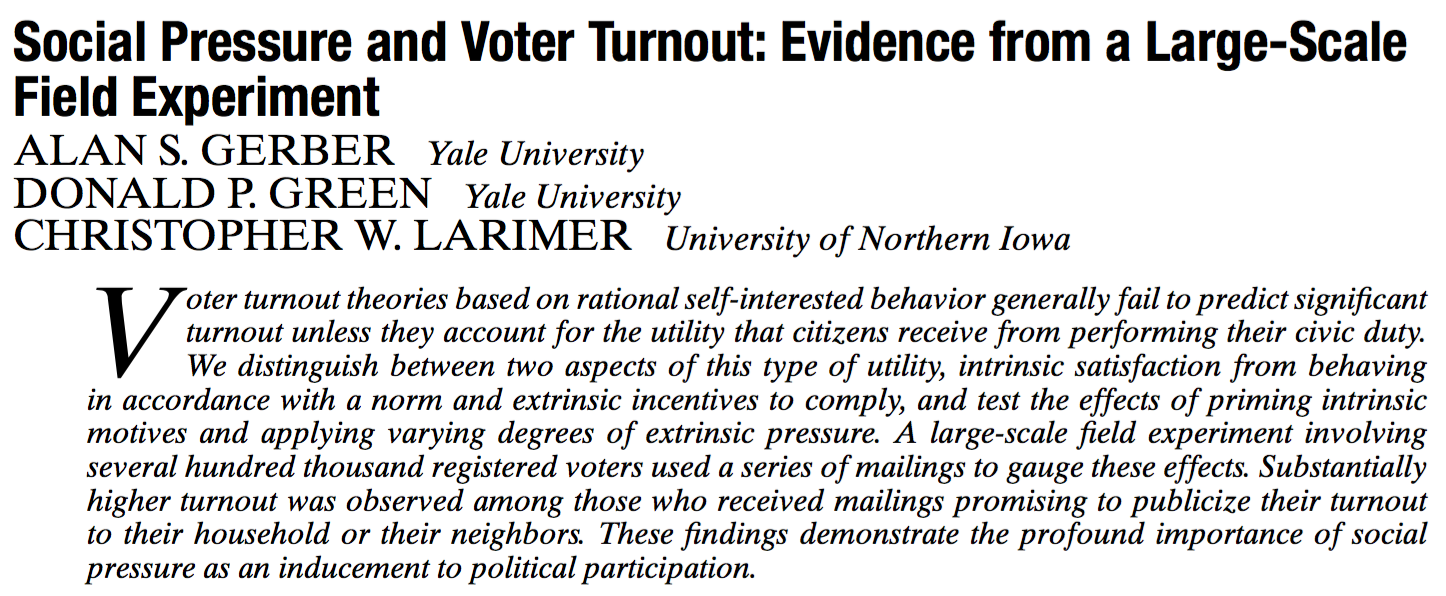
\includegraphics[width=4in]{figures/abstractGGL}
%\end{center}
%
%}
%
%%\frame{
%%\frametitle{The Civic Duty Treatment}
%%
%%\begin{center}
%%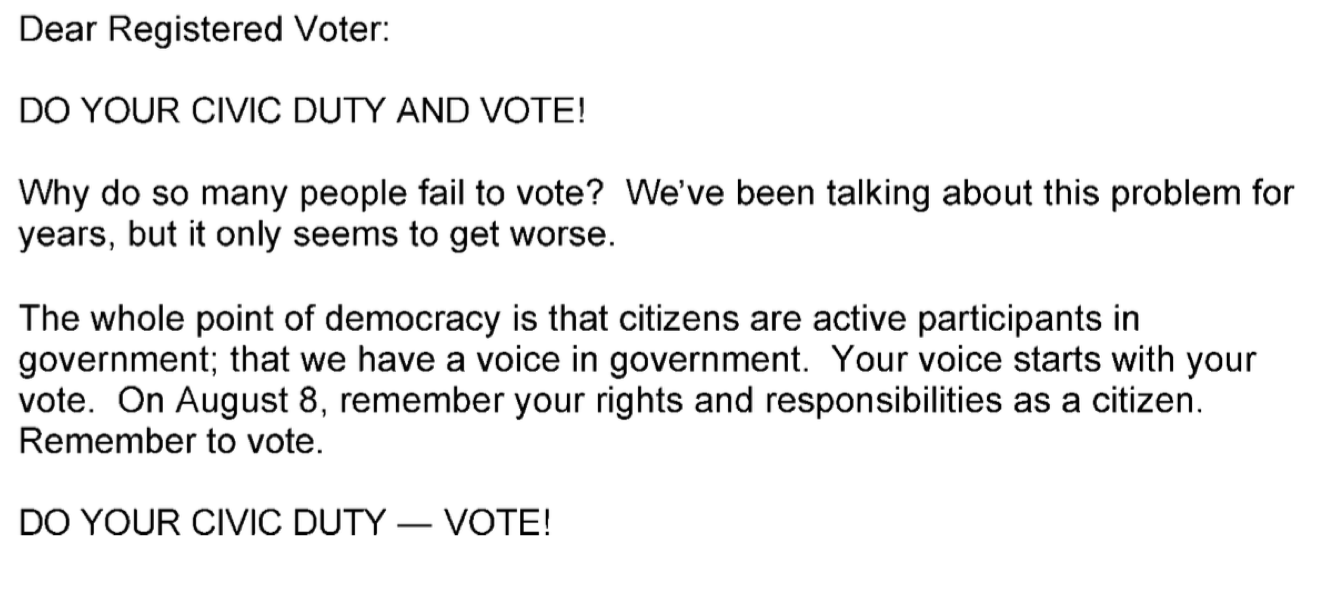
\includegraphics[width=4in]{figures/CivicDutyGGL}
%%\end{center}
%%
%%}
%%
%%\frame{
%%\frametitle{The Hawthorne Treatment}
%%
%%\begin{center}
%%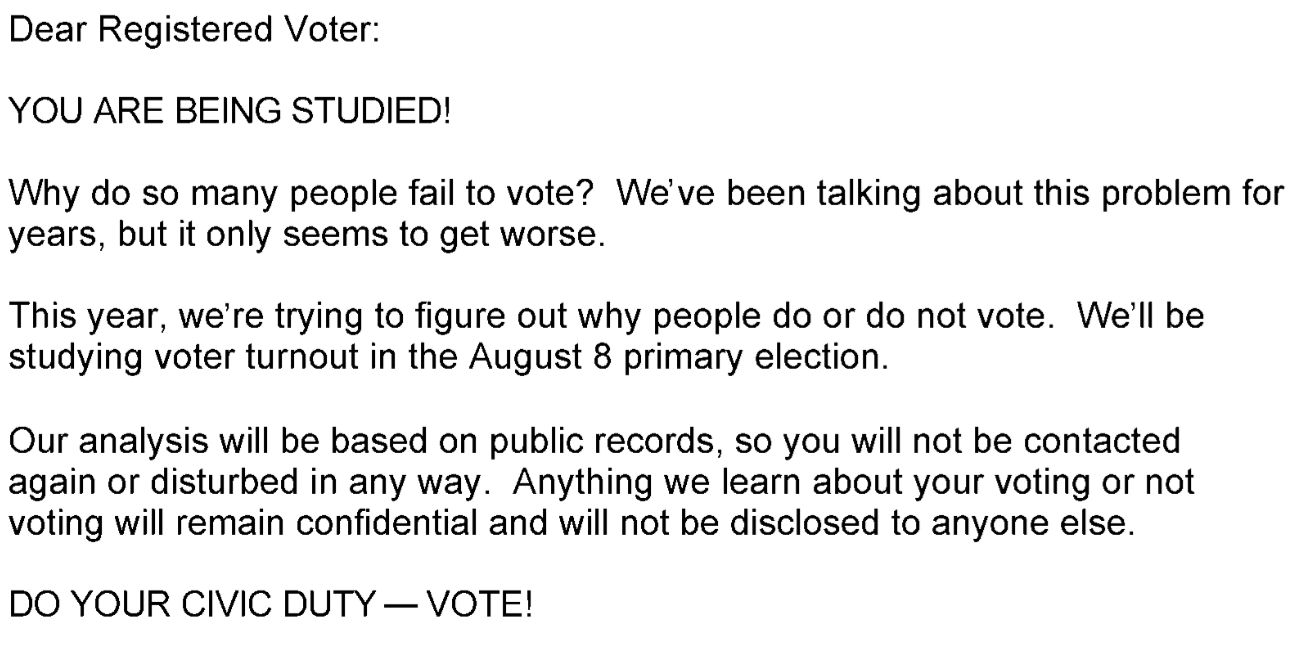
\includegraphics[width=4in]{figures/HawthorneGGL}
%%\end{center}
%%
%%}
%%
%%\frame{
%%\frametitle{The Self Treatment}
%%
%%\begin{center}
%%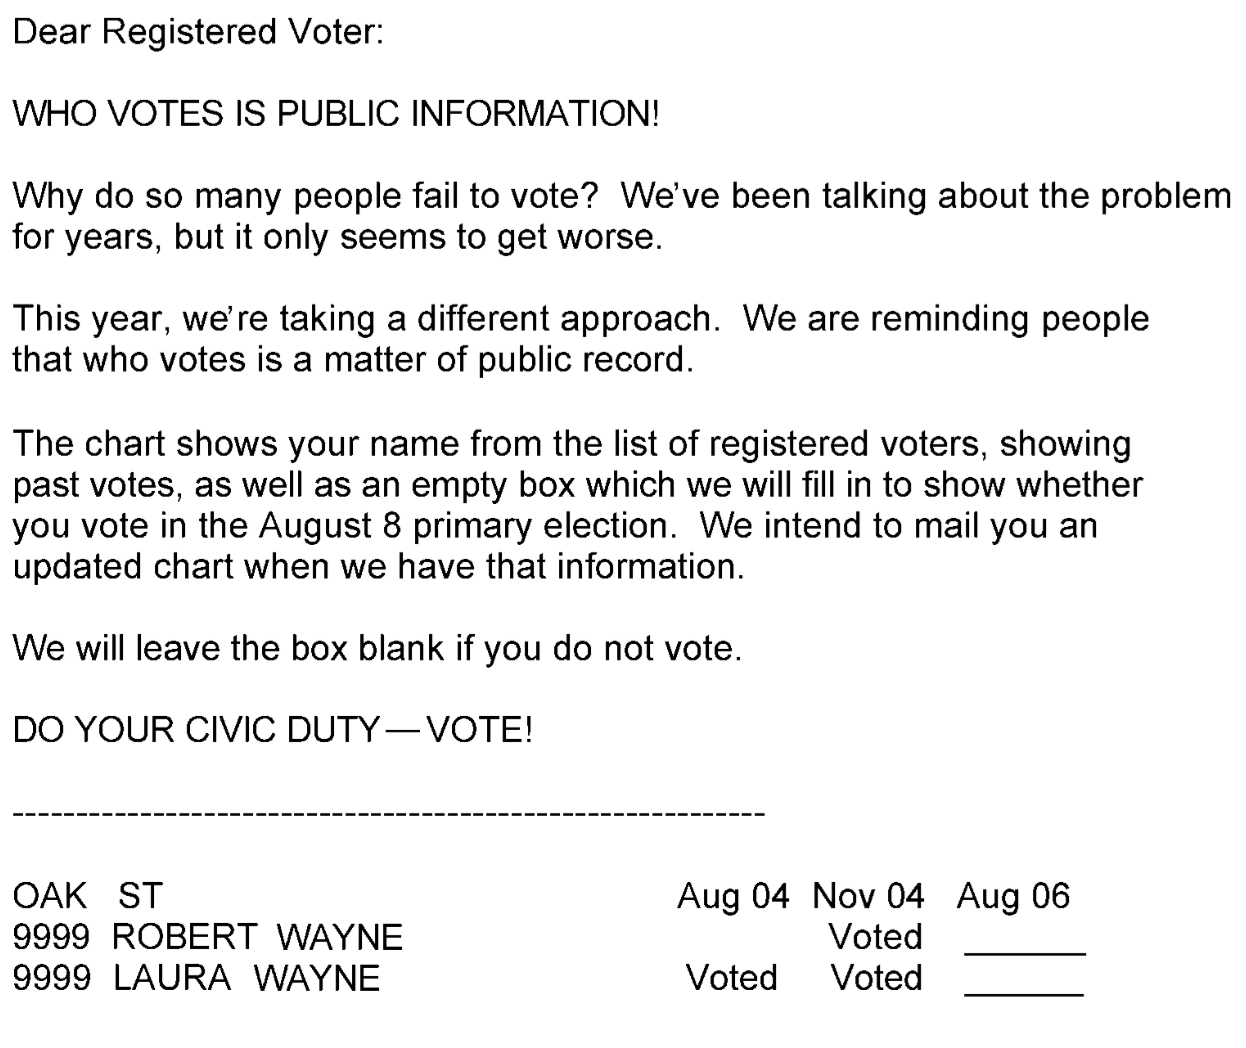
\includegraphics[width=3.5in]{figures/SelfGGL}
%%\end{center}
%%
%%}
%
%\frame{
%\frametitle{The Neighbors Treatment}
%
%\begin{center}
%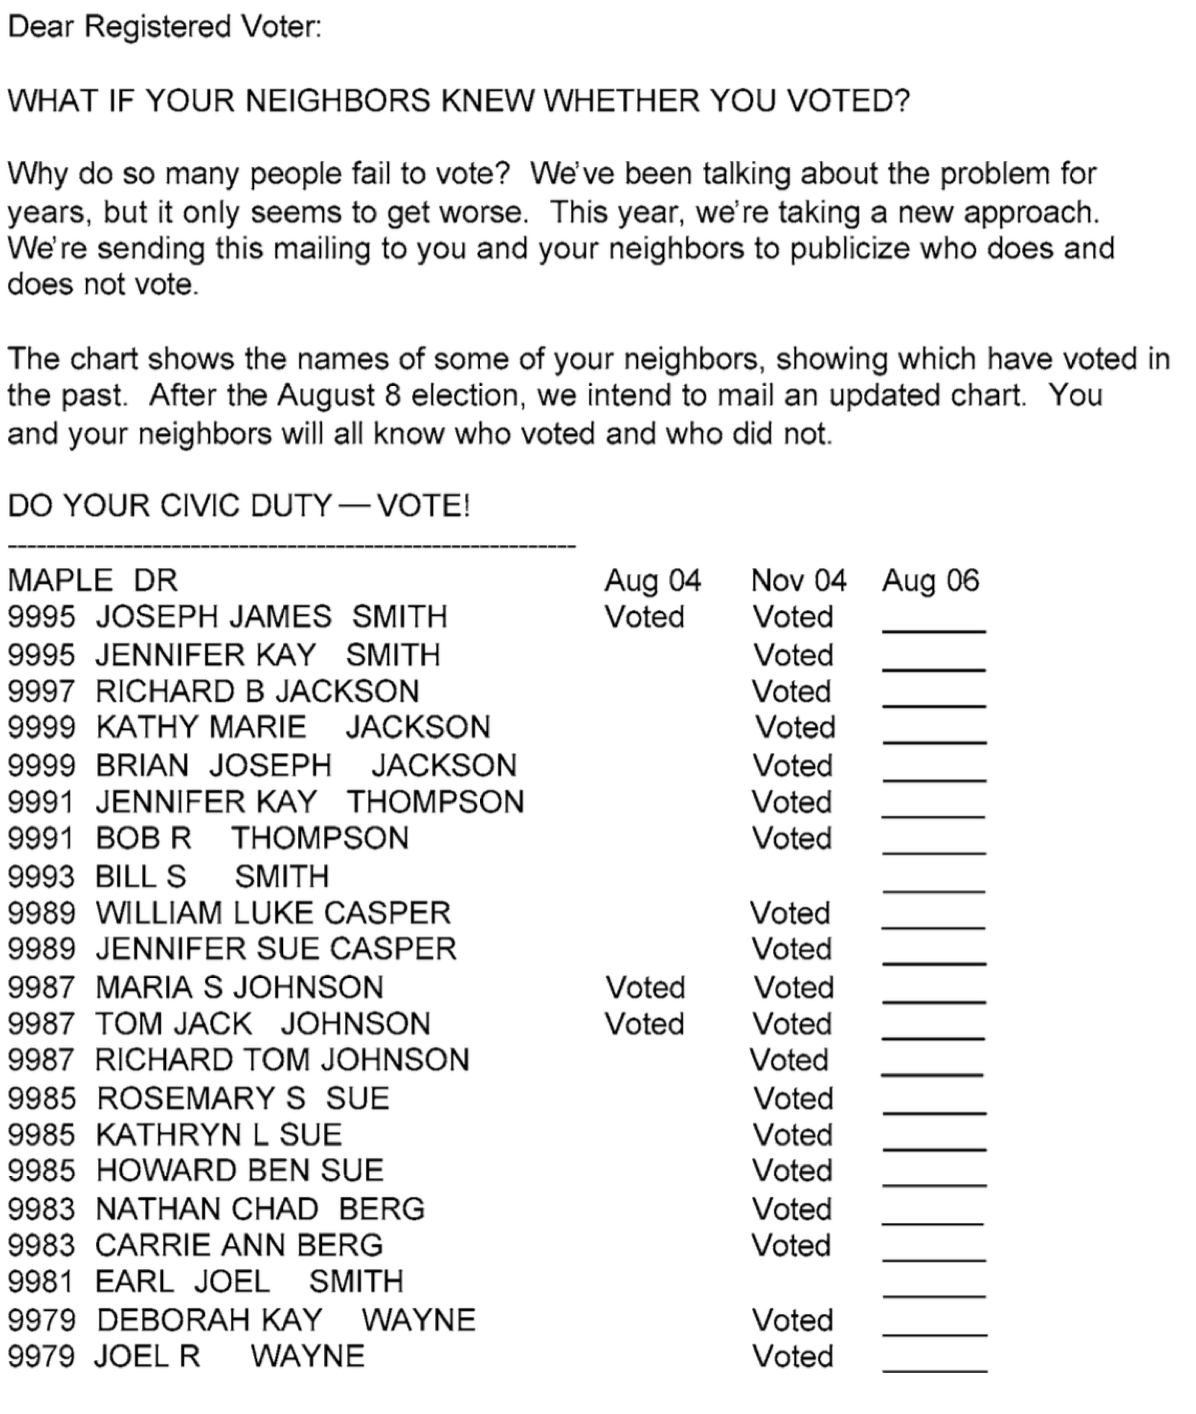
\includegraphics[width=3.5in]{figures/NeighborsGGL}
%\end{center}
%
%}
%
%\frame{
%\frametitle{Independence between Pre-treatment Variables and treatments in the GGL Experiment}
%
%\begin{center}
%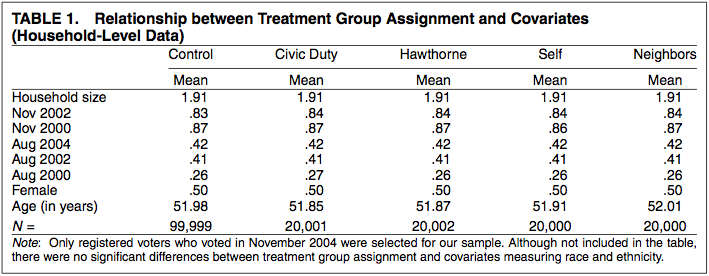
\includegraphics[width=4in]{lec15experiments/GGL}
%\end{center}
%
%}
%
%
%
%%\frame{
%%\frametitle{Including Covariates in the GGL Experiment}
%%
%%\begin{center}
%%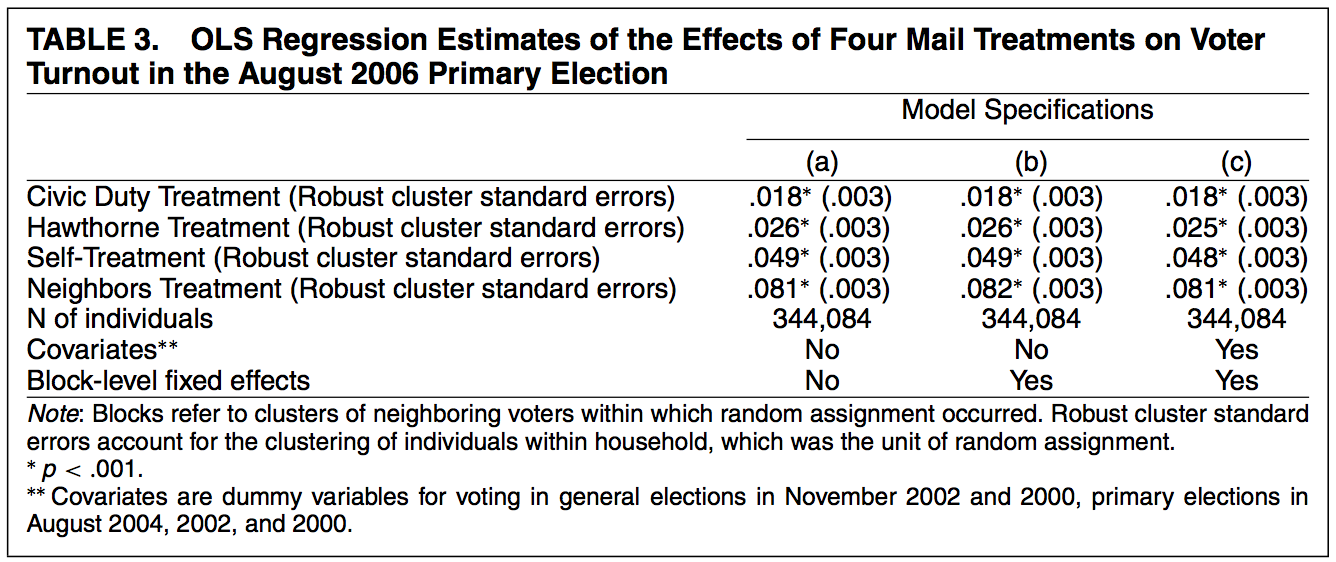
\includegraphics[width=4in]{lec15experiments/GGL2}
%%\end{center}
%%
%%}
%
%\frame{
%\frametitle{Warning: Independence only for pre-treatment X}
%
%\begin{itemize}
%\item If $X$ is affected by $D$, then the previous results will not hold.
%%\item Even though the $w=1$ rows are a random sample of the rows, $E[x|w=1] \ne E[x]$. 
%%\item Even though the $w=0$ rows are a random sample of the rows, $E[x|w=0] \ne E[x]$.
%%\item Therefore $E[x|w=1] \ne E[x|w=0]$.
%\item Suppose $Y=1$ indicates a heart attack, $D=1$ is a blood pressure medicine, and $X$ is post-treatment blood pressure. $X$ will be affected by $D$ and will therefore not be independent of $D$
%\end{itemize}
%
%}
%
%\frame{
%\frametitle{Including Covariates in the GGL Experiment}
%
%\begin{center}
%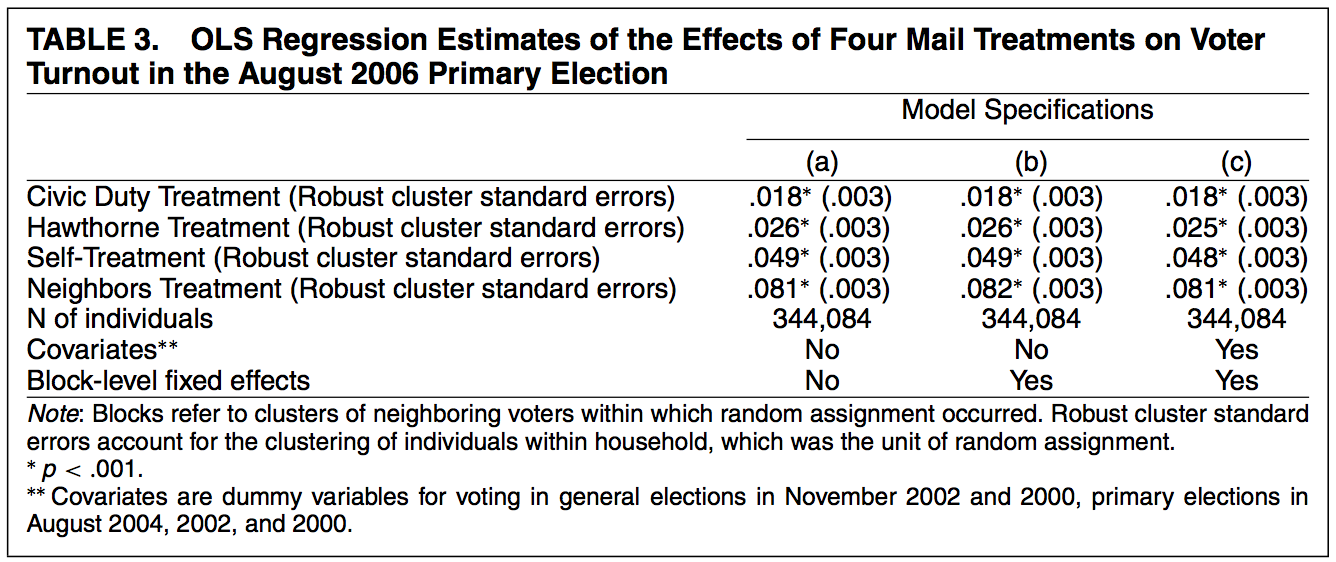
\includegraphics[width=4in]{lec15experiments/GGL2}
%\end{center}
%
%}
%
%
%\frame{
%\frametitle{SLR vs MLR with Randomized $D$}
%
%\begin{itemize}
%\item In very large samples, MLR will produce approximately the same answer as SLR for the ATE (e.g., social pressure). \pause
%\item In medium/large samples, (roughly $> 30$ d.f.), MLR will have small bias for the ATE but will generally be more efficient than SLR. \pause
%\item In small samples, the bias in multiple linear regression may be too much.  \pause
%\item The $X$ variables can include polynomials and interaction terms, but if $D$ is interacted with any $X$, then $\beta_D$ will no longer estimate ATE and we will need to use an APD. \pause
%\item This result holds for linear models used with limited dependent variables (LDV) such as the linear probability model when used with binary $Y$, but robust SEs must be used. 
%\end{itemize}
%
%}
%
%
%
%
%\frame{
%\frametitle{Interactions and LDVs}
%
%\begin{itemize}
%\item There can be small sample advantages to interacting $D$ with the $X$ variables but the APD should be used to estimate the ATE. \pause
%\item There can be small sample advantages to using LDV models such as logistic regression, but the APD should be used to estimate the ATE.
%\end{itemize}
%
%}
%
%

%\frame{
%
%\center
%\LARGE
%
%Conditionally Randomized Experiments 
%
%}

%\frame{
%\frametitle{Notation and Reading}
%
%For consistency, I'm using the notation from Wooldridge 3.7e and 7.6 in this section of the notes, but this material corresponds to the reading from Ch. 2.2-2.3 of Hernan and Robins \emph{What If}. 
%
%
%}

\frame{

Conditionally Randomized Experiments with a Discrete Blocking Variable

}

\frame{
\frametitle{Conditionally Randomized Experiment}


Suppose for one group/block/stratum ($\textcolor{green}{X=1}$) a coin was flipped to assign treatment to half of the units, and for another group/block stratum ($\textcolor{blue}{X=0}$), one out of four units was assigned to treatment. This is called a blocked, stratified, or conditionally randomized experiment. Essentially, we now have two experiments. 

\begin{center}
\begin{tabular}{cccc|ccc}
$i$ & $X_i$ & $D_i$ & $Y_i$ & $Y_i(1)$ & $Y_i(0)$ & $Y_i(1)-Y_i(0)$ \\
\hline
1 & \textcolor{blue}{0} &1 & 70 & \textcolor{blue}{70} & ? & ? \\
2 & \textcolor{green}{1} &1 & 80 & \textcolor{green}{80} & ? & ? \\
3 & \textcolor{blue}{0} & 0 & 60 & ? & \textcolor{blue}{60} &?\\
4 & \textcolor{green}{1} &0& 70 & ? & \textcolor{green}{70} & ? \\
5 & \textcolor{blue}{0} & 0&70 & ? & \textcolor{blue}{70} & ? \\
6 & \textcolor{blue}{0}& 0 & 80 & ? & \textcolor{blue}{80} & ? \\
\end{tabular}
\end{center}

}

\frame{
\frametitle{Conditionally Randomized Experiment}

Within each of our two groups ($\textcolor{blue}{X=0}$ and $\textcolor{green}{X=1}$), all the properties discussed in for randomized $D$ hold. 

\begin{center}

\begin{tabular}{cccc|ccc}
$i$ & $X_i$ & $D_i$ & $Y_i$ & $Y_i(1)$ & $Y_i(0)$ & $Y_i(1)-Y_i(0)$ \\
\hline
1 & \textcolor{blue}{0} &1 & 70 & \textcolor{blue}{70} & \alert{70} & \alert{0} \\
2 & \textcolor{green}{1} &1 & 80 & \textcolor{green}{80} & \alert{70} & \alert{10} \\
3 & \textcolor{blue}{0} & 0 & 60 & \alert{60} & \textcolor{blue}{60} & \alert{0}\\
4 & \textcolor{green}{1} &0& 70 & \alert{80} & \textcolor{green}{70} & \alert{10} \\
5 & \textcolor{blue}{0} & 0&70 & \alert{70} & \textcolor{blue}{70} & \alert{0} \\
6 & \textcolor{blue}{0}& 0 & 80 & \alert{80} & \textcolor{blue}{80} & \alert{0} \\
\end{tabular}\\
\alert{remember red numbers not observed}
\end{center}


\visible<1-2>{What is the average $Y_i(1)$ among the $X=0$ subjects?} 
\visible<2>{$$
\frac{\textcolor{blue}{70} +\alert{60} +\alert{70} + \alert{80}}{4}  = 70
$$}
\vspace{-2.4cm}

\visible<3-4>{What is the average $Y_i(1)$ among the $X=0$, $D=1$ subjects?} 
\visible<4>{$$
\frac{\textcolor{blue}{70} }{1}  = 70
$$}
\vspace{-2.4cm}

\visible<5-6>{What is the average $Y_i(0)$ among the $X=0$ subjects?} 
\visible<6>{$$
\frac{\textcolor{red}{70} +\textcolor{blue}{60} +\textcolor{blue}{70}+\textcolor{blue}{80}}{4}  = 70
$$}
\vspace{-2.4cm}

\visible<7-8>{What is the average $Y_i(0)$ among the $X=0$, $D=0$ subjects?} 
\visible<8>{$$
\frac{\textcolor{blue}{60} +\textcolor{blue}{70}+\textcolor{blue}{80}}{3}  = 70
$$}

}

\frame{
\frametitle{Conditional ATE for $\textcolor{blue}{X=0}$}

Because we have a randomized experiment within the  $\textcolor{blue}{X=0}$ group and because of the linearity of expectations, the SLR slope (difference in means) among the $\textcolor{blue}{X=0}$ group provides an unbiased estimator of the conditional average treatment effect ($CATE_{x=0}$). 

\begin{align*}
&\frac{\textcolor{blue}{70} }{1}  - \frac{\textcolor{blue}{60} +\textcolor{blue}{70}+\textcolor{blue}{80}}{3} \\
&= \frac{\textcolor{blue}{70} +\alert{60} +\alert{70} + \alert{80}}{4} - \frac{\textcolor{red}{70} +\textcolor{blue}{60} +\textcolor{blue}{70}+\textcolor{blue}{80}}{4} \\
&= \frac{\alert{0} +\alert{0} +\alert{0} + \alert{0}}{4}
\end{align*}


}



\frame{
\frametitle{Conditionally Randomized Experiment}

Within the $\textcolor{green}{X=1}$ group, all the properties discussed for randomized $D$ hold.

\begin{center}
\begin{tabular}{cccc|ccc}
$i$ & $X_i$ & $D_i$ & $Y_i$ & $Y_i(1)$ & $Y_i(0)$ & $Y_i(1)-Y_i(0)$ \\
\hline
1 & \textcolor{blue}{0} &1 & 70 & \textcolor{blue}{70} & \alert{70} & \alert{0} \\
2 & \textcolor{green}{1} &1 & 80 & \textcolor{green}{80} & \alert{70} & \alert{10} \\
3 & \textcolor{blue}{0} & 0 & 60 & \alert{60} & \textcolor{blue}{60} & \alert{0}\\
4 & \textcolor{green}{1} &0& 70 & \alert{80} & \textcolor{green}{70} & \alert{10} \\
5 & \textcolor{blue}{0} & 0&70 & \alert{70} & \textcolor{blue}{70} & \alert{0} \\
6 & \textcolor{blue}{0}& 0 & 80 & \alert{80} & \textcolor{blue}{80} & \alert{0} \\
\end{tabular}
\end{center}


\visible<1-2>{What is the average $Y_i(1)$ among the $X=1$ subjects?} 
\visible<2>{$$
\frac{\textcolor{green}{80} +\alert{80} }{2}  = 80
$$}
\vspace{-2.4cm}

\visible<3-4>{What is the average $Y_i(1)$ among the $X=1$, $D=1$ subjects?} 
\visible<4>{$$
\frac{\textcolor{green}{80}}{1}  = 80
$$}
\vspace{-2.4cm}

\visible<5-6>{What is the average $Y_i(0)$ among the $X=1$ subjects?} 
\visible<6>{$$
\frac{\alert{70}  + \textcolor{green}{70}}{2}  = 70
$$}
\vspace{-2.4cm}

\visible<7-8>{What is the average $Y_i(0)$ among the $X=1$, $D=0$ subjects?} 
\visible<8>{$$
\frac{\textcolor{green}{70}}{1}  = 70
$$}

}

\frame{
\frametitle{Conditional ATE for $\textcolor{green}{X=1}$}

Because we have a randomized experiment within the $\textcolor{green}{X=1}$ group and because of the linearity of expectations, the SLR slope (difference in means) among the $\textcolor{green}{X=1}$ group provides an unbiased estimator of the conditional average treatment effect ($CATE_{x=1}$). 

\begin{align*}
&\frac{\textcolor{green}{80} }{1}  - \frac{\textcolor{green}{70} }{1} \\
&=\frac{\textcolor{green}{80} +\alert{80} }{2} - \frac{\alert{70}  + \textcolor{green}{70}}{2} \\
&= \frac{\alert{10} +\alert{10}}{2}
\end{align*}


}




\frame{
\frametitle{Standardization via APD}


If we average the $CATE_{x=0}$ and $CATE_{x=1}$ by the proportion in each group/block/stratum, this is an APD, which gives us the ATE. In epidemiology, this is known as standardization.

\begin{center}
\begin{tabular}{cccc|ccc}
$i$ & $X_i$ & $D_i$ & $Y_i$ & $Y_i(1)$ & $Y_i(0)$ & $Y_i(1)-Y_i(0)$ \\
\hline
1 & \textcolor{blue}{0} &1 & 70 & \textcolor{blue}{70} & ? & ? \\
2 & \textcolor{green}{1} &1 & 80 & \textcolor{green}{80} & ? & ? \\
3 & \textcolor{blue}{0} & 0 & 60 & ? & \textcolor{blue}{60} &?\\
4 & \textcolor{green}{1} &0& 70 & ? & \textcolor{green}{70} & ? \\
5 & \textcolor{blue}{0} & 0&70 & ? & \textcolor{blue}{70} & ? \\
6 & \textcolor{blue}{0}& 0 & 80 & ? & \textcolor{blue}{80} & ? \\
\end{tabular}
\end{center}



\begin{align*}
\textcolor{blue}{\frac{4}{6}} \cdot \left\{\frac{70}{1} -  \frac{60+70+80}{3}\right\} &+ \textcolor{green}{\frac{2}{6}} \cdot \left\{\frac{80}{1} -  \frac{70}{1}\right\} \\
&= \frac{20}{6}
\end{align*}
}


\frame{
\frametitle{Standardization via APD}


If we average the $CATE_{x=0}$ and $CATE_{x=1}$ by the proportion in each group/block/stratum, this is an APD, which gives us the ATE. In epidemiology, this is known as standardization.

\begin{center}
\begin{tabular}{cccc|ccc}
$i$ & $X_i$ & $D_i$ & $Y_i$ & $Y_i(1)$ & $Y_i(0)$ & $Y_i(1)-Y_i(0)$ \\
\hline
1 & \textcolor{blue}{0} &1 & 70 & \textcolor{blue}{70} & \alert{70} & \alert{0} \\
2 & \textcolor{green}{1} &1 & 80 & \textcolor{green}{80} & \alert{70} & \alert{10} \\
3 & \textcolor{blue}{0} & 0 & 60 & \alert{60} & \textcolor{blue}{60} & \alert{0}\\
4 & \textcolor{green}{1} &0& 70 & \alert{80} & \textcolor{green}{70} & \alert{10} \\
5 & \textcolor{blue}{0} & 0&70 & \alert{70} & \textcolor{blue}{70} & \alert{0} \\
6 & \textcolor{blue}{0}& 0 & 80 & \alert{80} & \textcolor{blue}{80} & \alert{0} \\
\end{tabular}
\end{center}



\begin{align*}
\textcolor{blue}{\frac{4}{6}} \cdot \left\{\frac{70}{1} -  \frac{60+70+80}{3}\right\} &+ \textcolor{green}{\frac{2}{6}} \cdot \left\{\frac{80}{1} -  \frac{70}{1}\right\} \\
&= \frac{20}{6} = \frac{\alert{10}+\alert{10}}{6}
\end{align*}
}

\frame{

\begin{itemize}
\item The ATE estimation method on the previous slide is equivalent to an APD with an interactive linear model ($Y \sim D + X + D:X$ in R formula notation).
\item Many researchers would simply estimate the effect with an additive linear model ($Y \sim D + X$ in R formula notation), but this would target a weighted average treatment effect.
\end{itemize}

}

\frame{
\frametitle{Omitted variable bias with SLR}


If we ignore the groups, and run an SLR on the entire data, we get omitted variable bias.

\begin{center}
\begin{tabular}{cccc|ccc}
$i$ & $X_i$ & $T_i$ & $Y_i$ & $Y_i(1)$ & $Y_i(0)$ & $Y_i(1)-Y_i(0)$ \\
\hline
1 & \textcolor{blue}{0} &1 & 70 & \textcolor{blue}{70} & \alert{70} & \alert{0} \\
2 & \textcolor{green}{1} &1 & 80 & \textcolor{green}{80} & \alert{70} & \alert{10} \\
3 & \textcolor{blue}{0} & 0 & 60 & \alert{60} & \textcolor{blue}{60} & \alert{0}\\
4 & \textcolor{green}{1} &0& 70 & \alert{80} & \textcolor{green}{70} & \alert{10} \\
5 & \textcolor{blue}{0} & 0&70 & \alert{70} & \textcolor{blue}{70} & \alert{0} \\
6 & \textcolor{blue}{0}& 0 & 80 & \alert{80} & \textcolor{blue}{80} & \alert{0} \\
\end{tabular}
\end{center}


\visible<1-2>{What is the average $Y_i(1) - Y_i(0)$?} 
\visible<2>{
\begin{align*}
\frac{\alert{0} + \alert{10} + \alert{0} +  \alert{10} +\alert{0} +\alert{0}}{6}  &= \frac{20}{6}\\
&\approx 3.3\\
 &\ne \frac{\textcolor{blue}{70} +\textcolor{green}{80} }{2} -  \frac{\textcolor{blue}{60} +\textcolor{green}{70} +  \textcolor{blue}{70} +\textcolor{blue}{80} }{4}
\end{align*}}

}

\frame{
\frametitle{Summary of Conditionally Randomized Experiments}

\begin{itemize}
\item A conditionally randomized experiment (with a discrete blocking variable) can be analyzed as multiple experiments and these results can be combined with standardization (an APD). 
\item A additive MLR of $Y$ on $D$ and $X$ will produce a weighted average treatment effect.
\item If you ignore the groups in a conditionally randomized experiment, and the probability of treatment assignment is different in the groups, then you will induce omitted variable bias. 
\end{itemize}

}

\frame{
\frametitle{Up Next}

\begin{itemize}
\item What about randomization conditional on a continuous covariate and/or many covariates? 
\item Many non-experimental studies can be thought of as approximating a conditionally randomized experiment. 
\item We will use APDs to estimate the ATE in these studies (e.g. effect of runoff elections on number of presidential candidates).
\item Need to worry about omitted variable bias. 
\end{itemize}

}

\frame{
\frametitle{Neto and Cox (1997) Table 3 Data}

\begin{figure}[ht]
  \begin{center}
    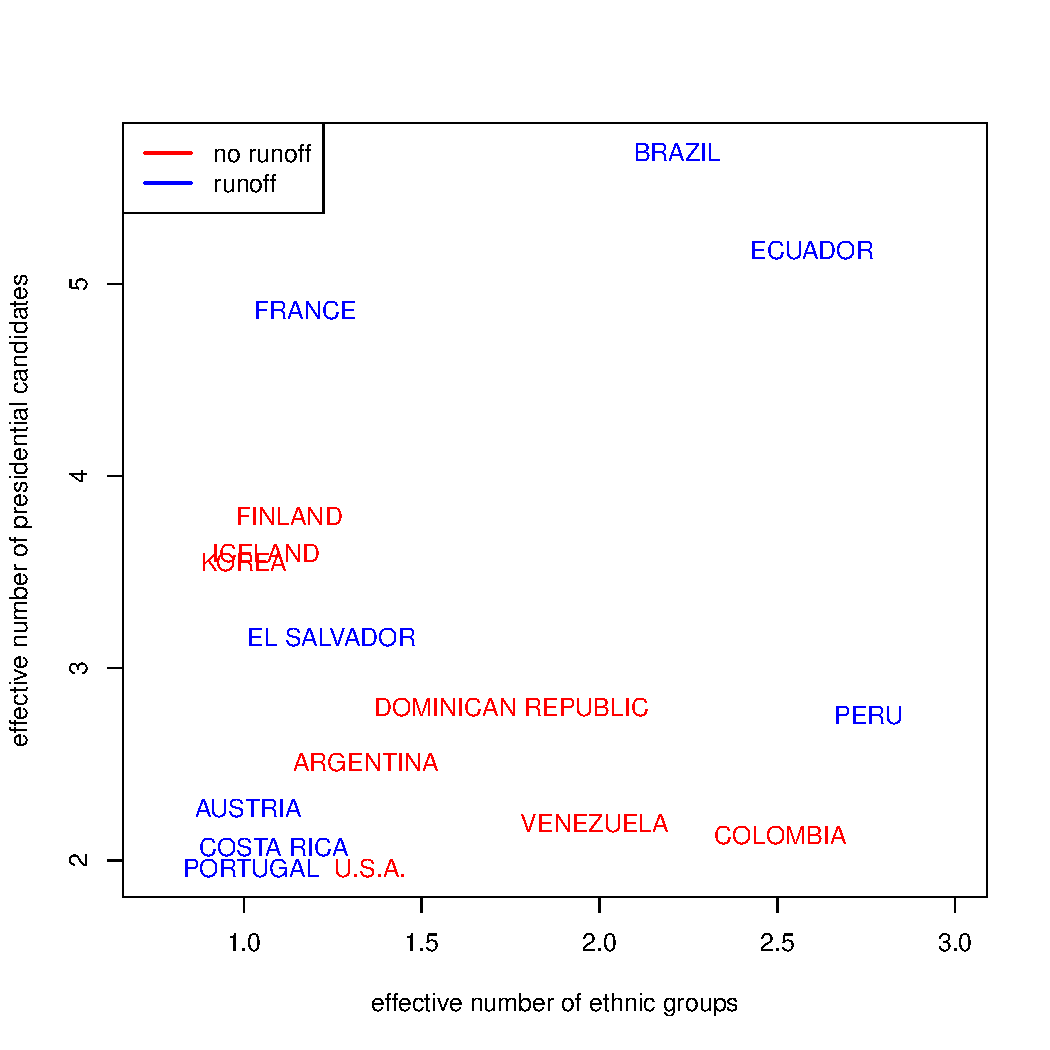
\includegraphics[height=3in]{figures/p1.pdf}
  \end{center}
  \vspace{-0.275in}
\end{figure}

}

\frame{

Remember the estimation of APDs for a binary covariate.

}

\frame{
\frametitle{Average Partial Derivative (Runoff) in Additive Model}

\begin{figure}[ht]
  \begin{center}
    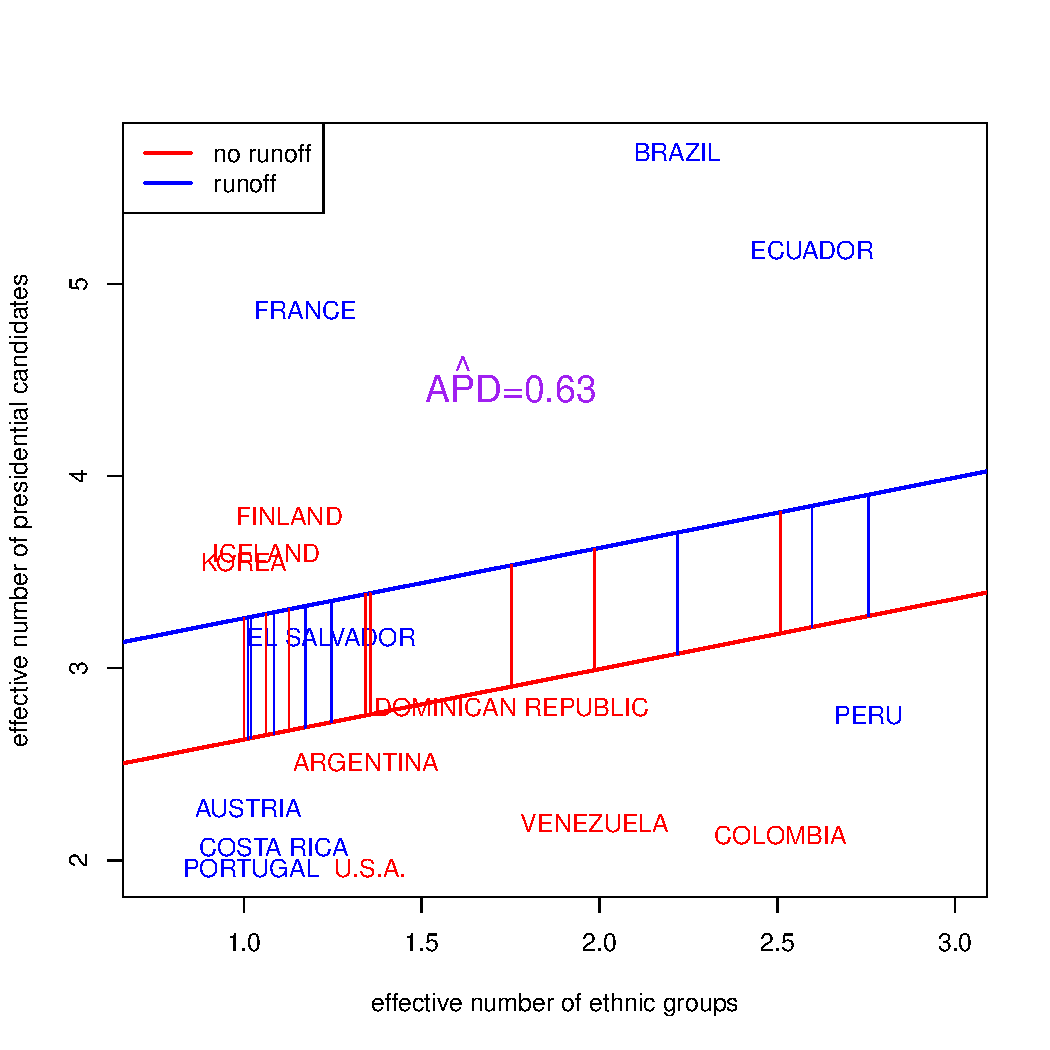
\includegraphics[height=3in]{figures/p2b.pdf}
  \end{center}
  \vspace{-0.275in}
\end{figure}

}

\frame{
\frametitle{APD in Interactive/Unpooled Linear Model}

\begin{figure}[ht]
  \begin{center}
    \includegraphics<1>[height=3in]{figures/p3.pdf}
    \includegraphics<2>[height=3in]{figures/p4b.pdf}
  \end{center}
  \vspace{-0.275in}
\end{figure}

}

\frame{
\frametitle{APD in Additive Quadratic Models}

\begin{figure}[ht]
  \begin{center}
    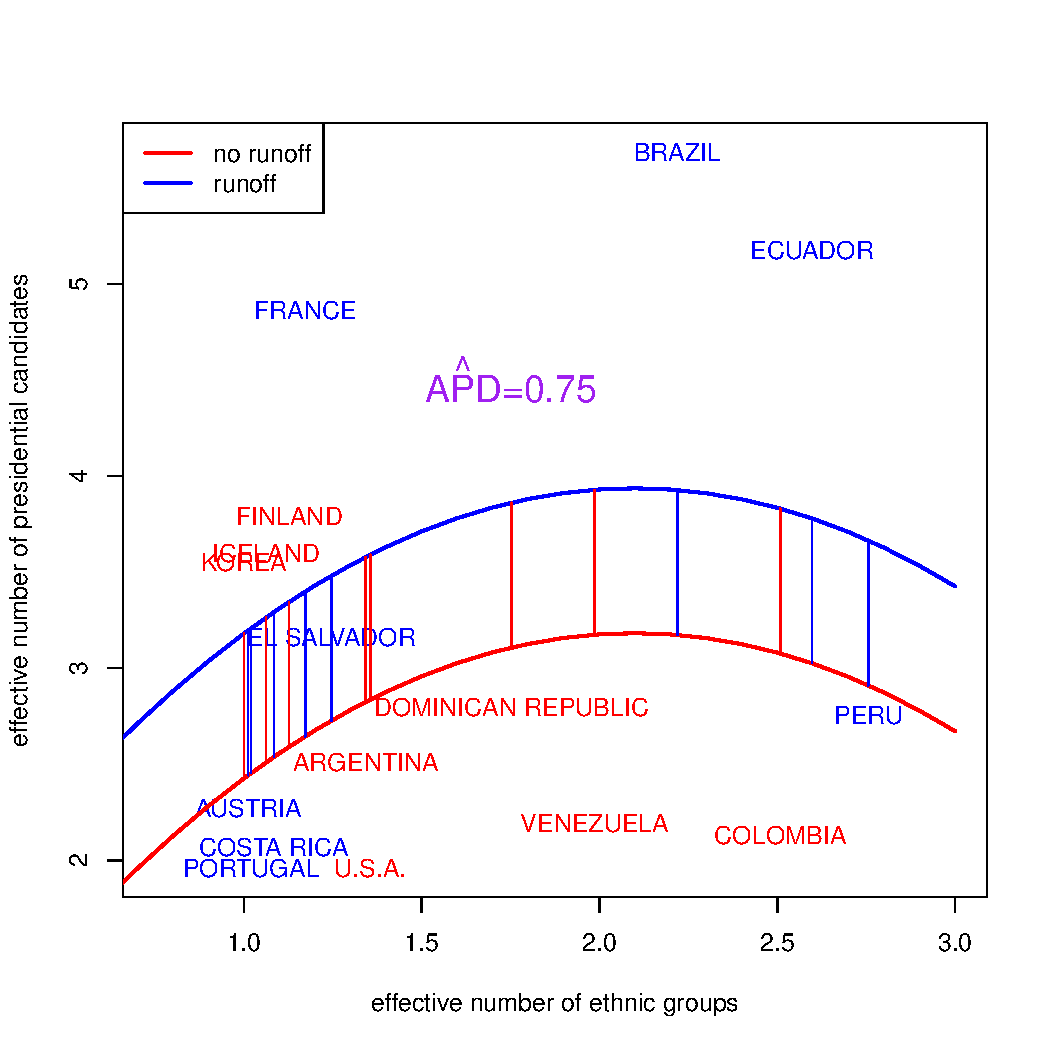
\includegraphics[height=3in]{figures/p13b.pdf}
  \end{center}
  \vspace{-0.275in}
\end{figure}

}


\frame{
\frametitle{APD in Interactive/Unpooled Quadratic}

\begin{figure}[ht]
  \begin{center}
    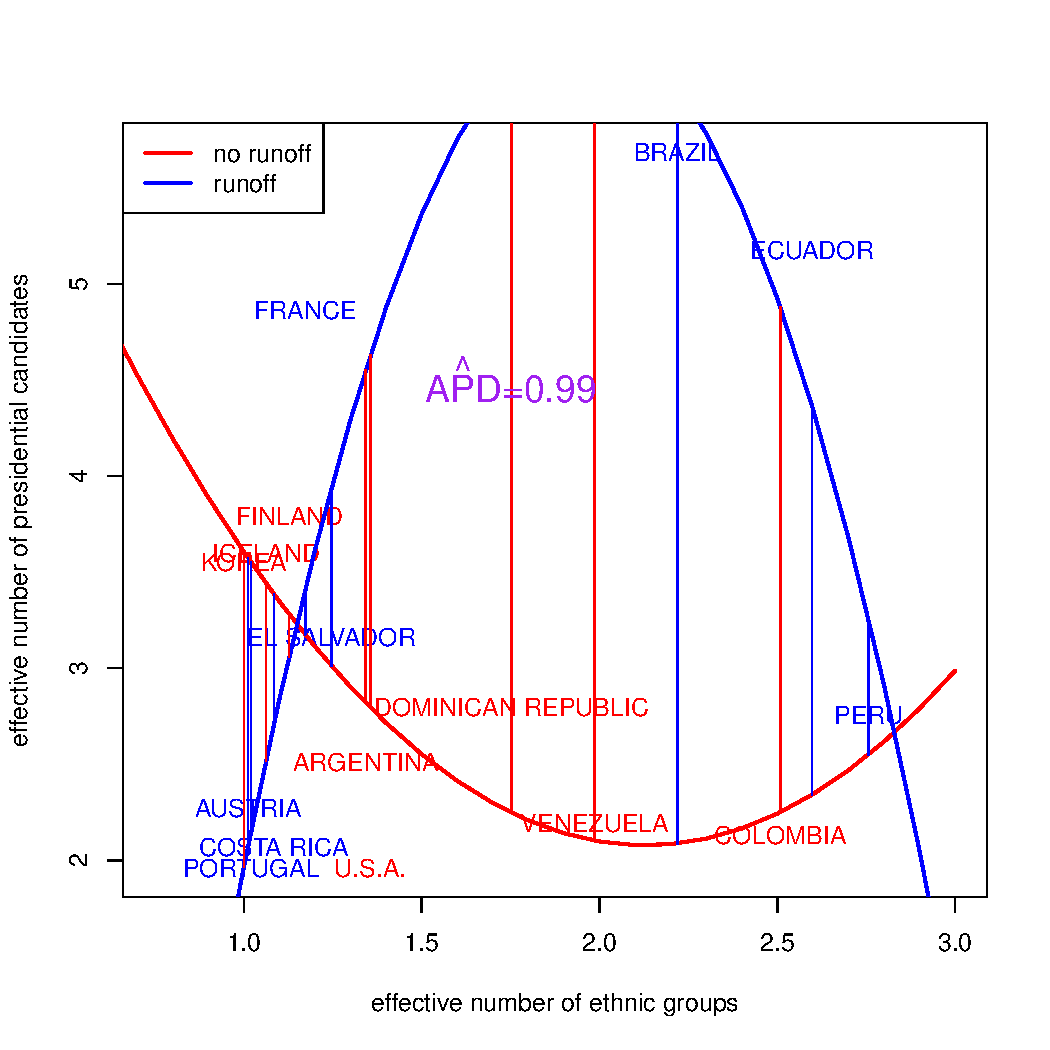
\includegraphics[height=3in]{figures/p13c.pdf}
  \end{center}
  \vspace{-0.275in}
\end{figure}

}

%\frame{
%\frametitle{APD in Unpooled Local Regression}
%
%\begin{figure}[ht]
%  \begin{center}
%    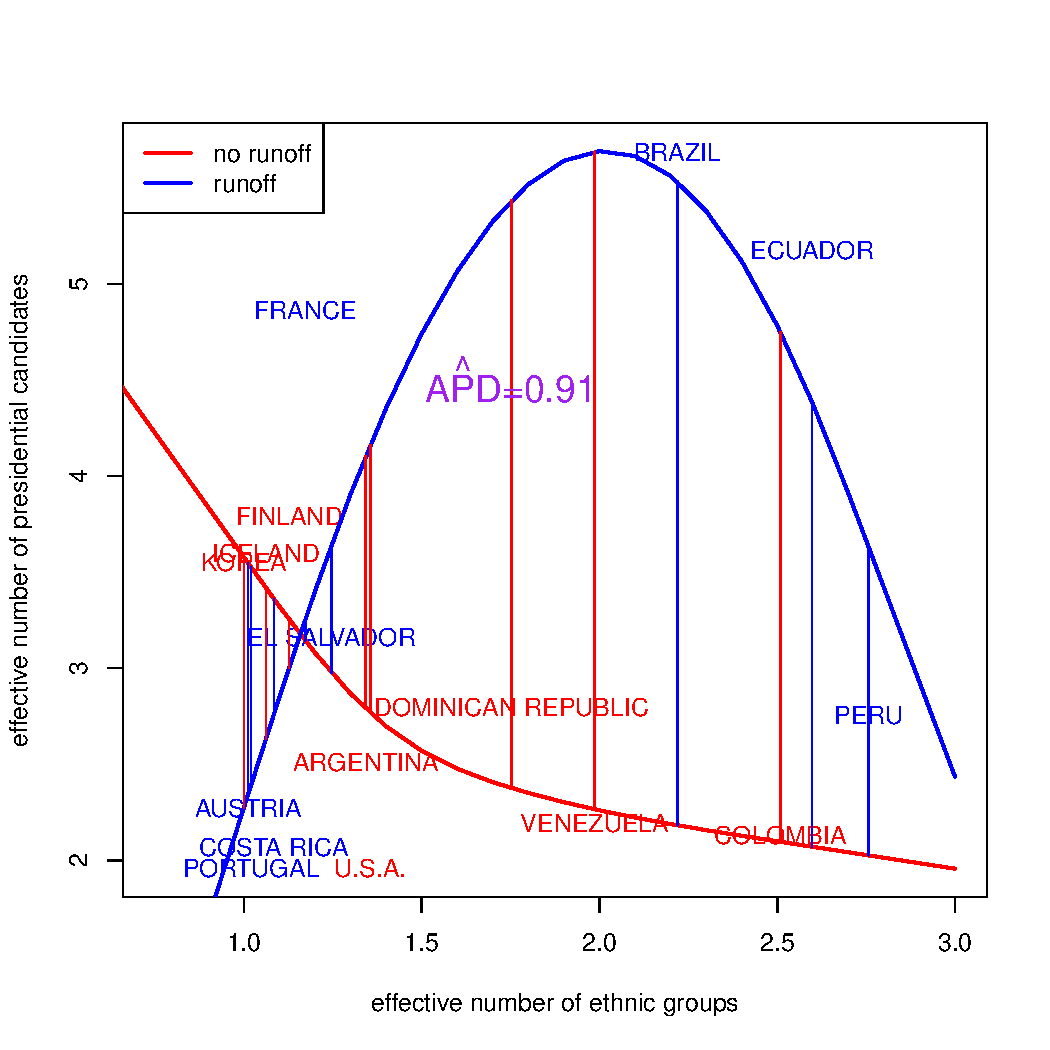
\includegraphics[height=3in]{figures/p15d.pdf}
%  \end{center}
%  \vspace{-0.275in}
%\end{figure}
%
%}

\frame{

Let's think about the Neto and Cox data causally, and start with the heroic assumption that whether a country has a runoff election is randomly assigned, conditional on how many ethnic groups they have. 

}

\frame{
\frametitle{Neto and Cox (1997) Table 3 Data}

\begin{figure}[ht]
  \begin{center}
    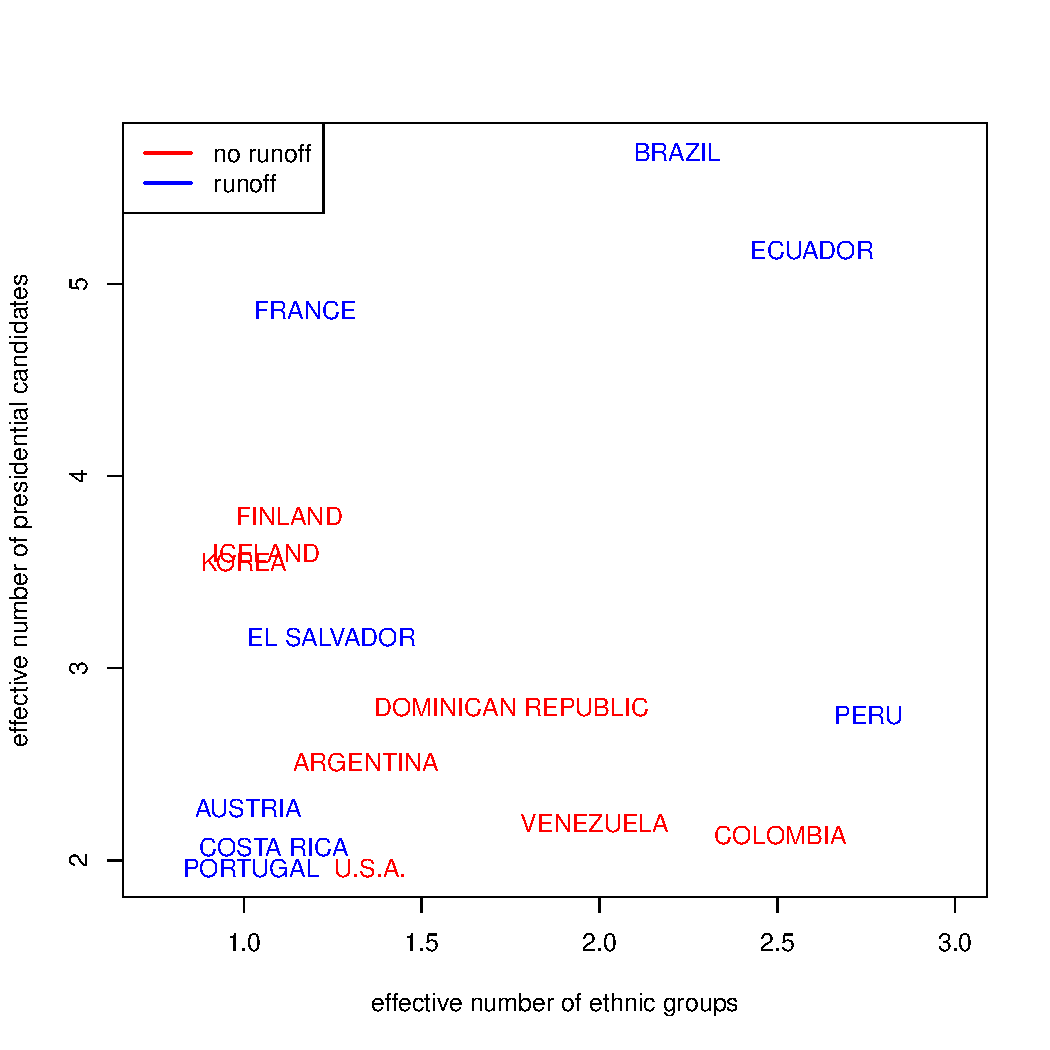
\includegraphics[height=3in]{figures/p1.pdf}
  \end{center}
  \vspace{-0.275in}
\end{figure}

}

\frame{
\frametitle{Focus on the no runoff countries}

\begin{figure}[ht]
  \begin{center}
    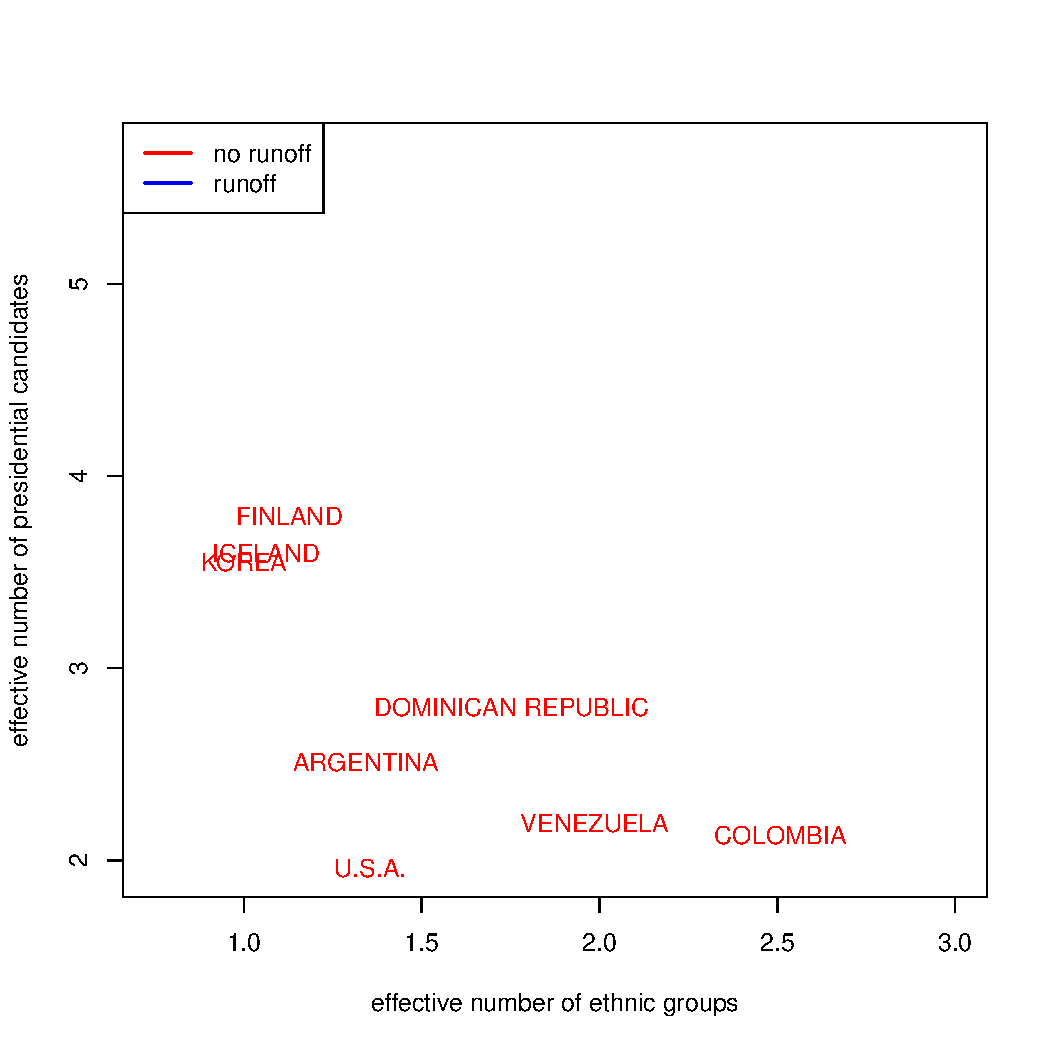
\includegraphics[height=3in]{figures/p1a.pdf}
  \end{center}
  \vspace{-0.275in}
\end{figure}

}

\frame{
\frametitle{Which potential outcome are we observing?}

\begin{figure}[ht]
  \begin{center}
    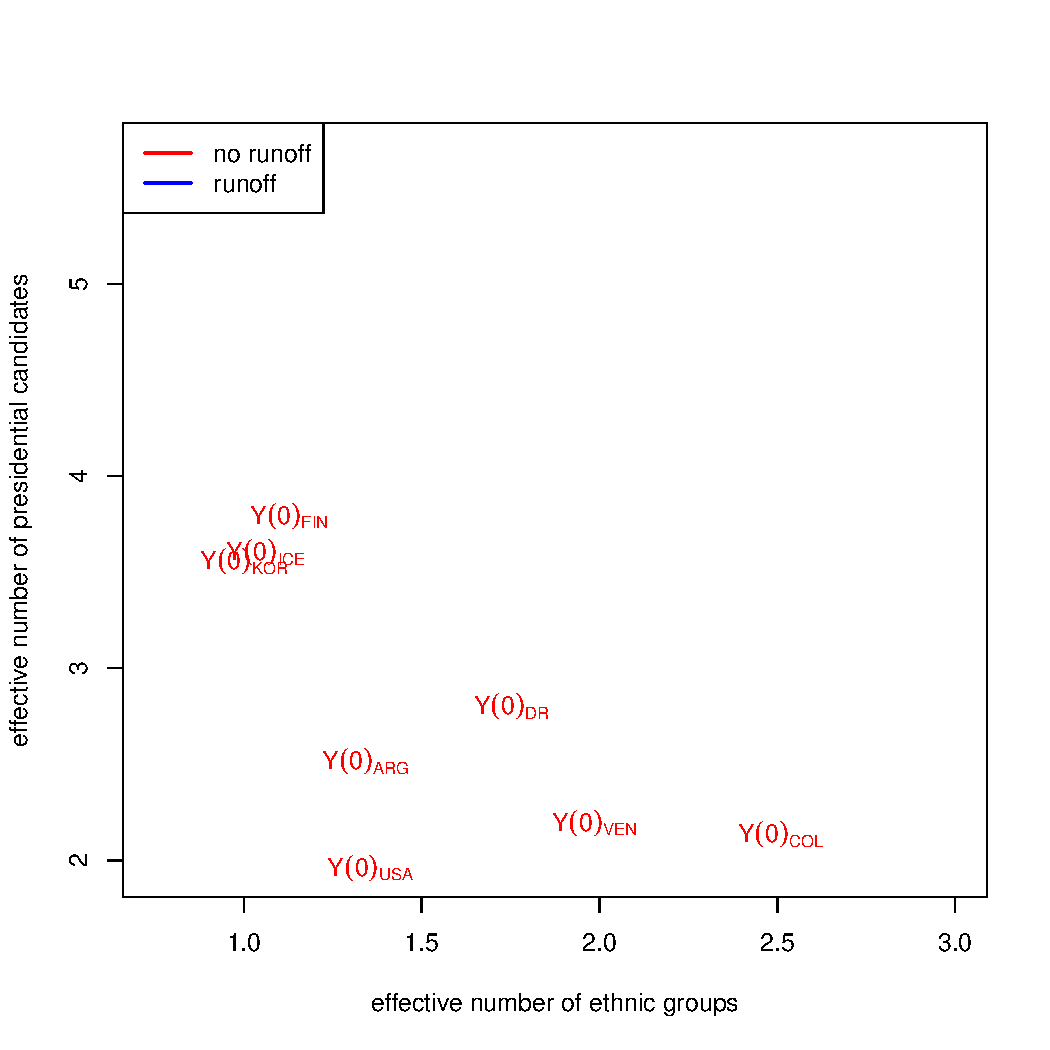
\includegraphics[height=3in]{figures/p1b.pdf}
  \end{center}
  \vspace{-0.275in}
\end{figure}

}

\frame{
\frametitle{Bringing back runoff countries}

\begin{figure}[ht]
  \begin{center}
    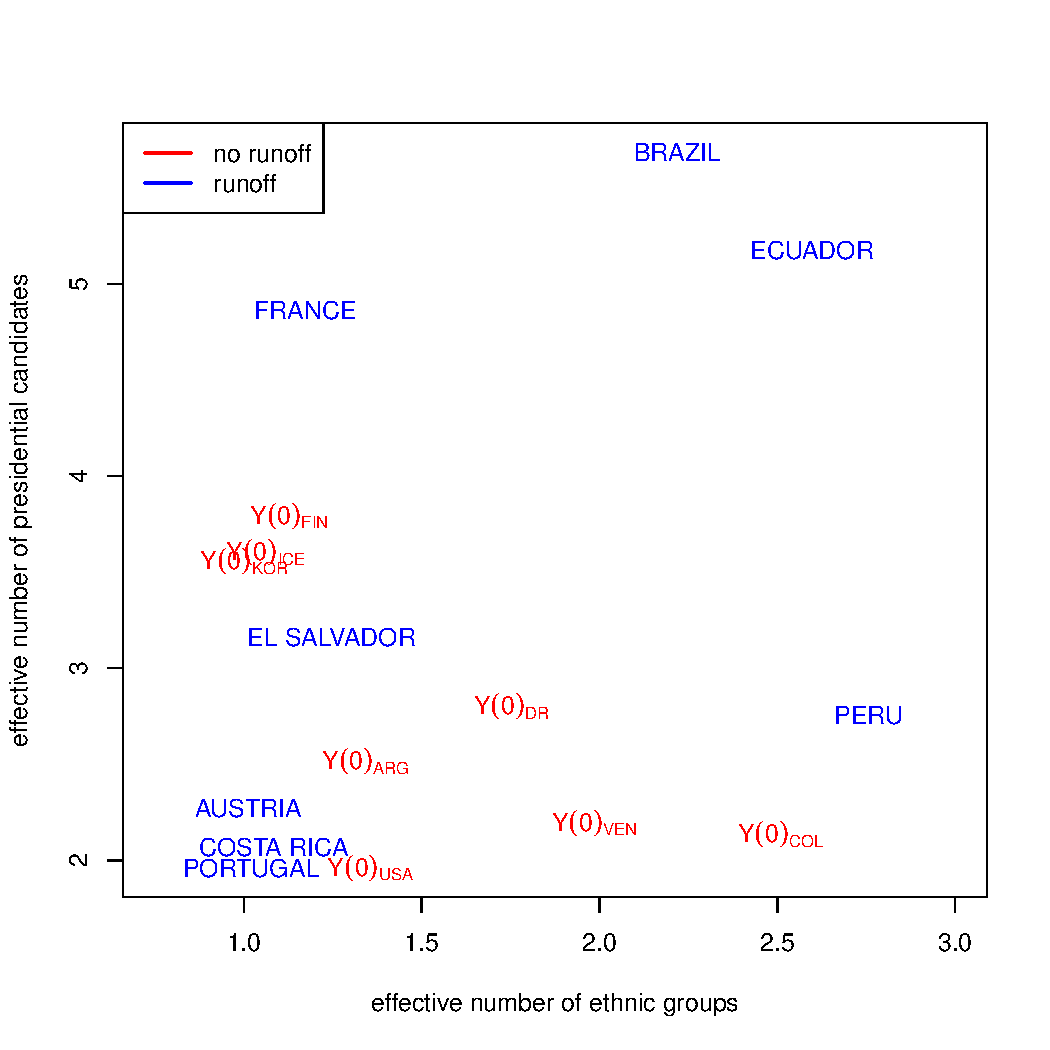
\includegraphics[height=3in]{figures/p1c.pdf}
  \end{center}
  \vspace{-0.275in}
\end{figure}

}

\frame{
\frametitle{How to impute $Y(1)$ for no runoff countries?}

\begin{figure}[ht]
  \begin{center}
    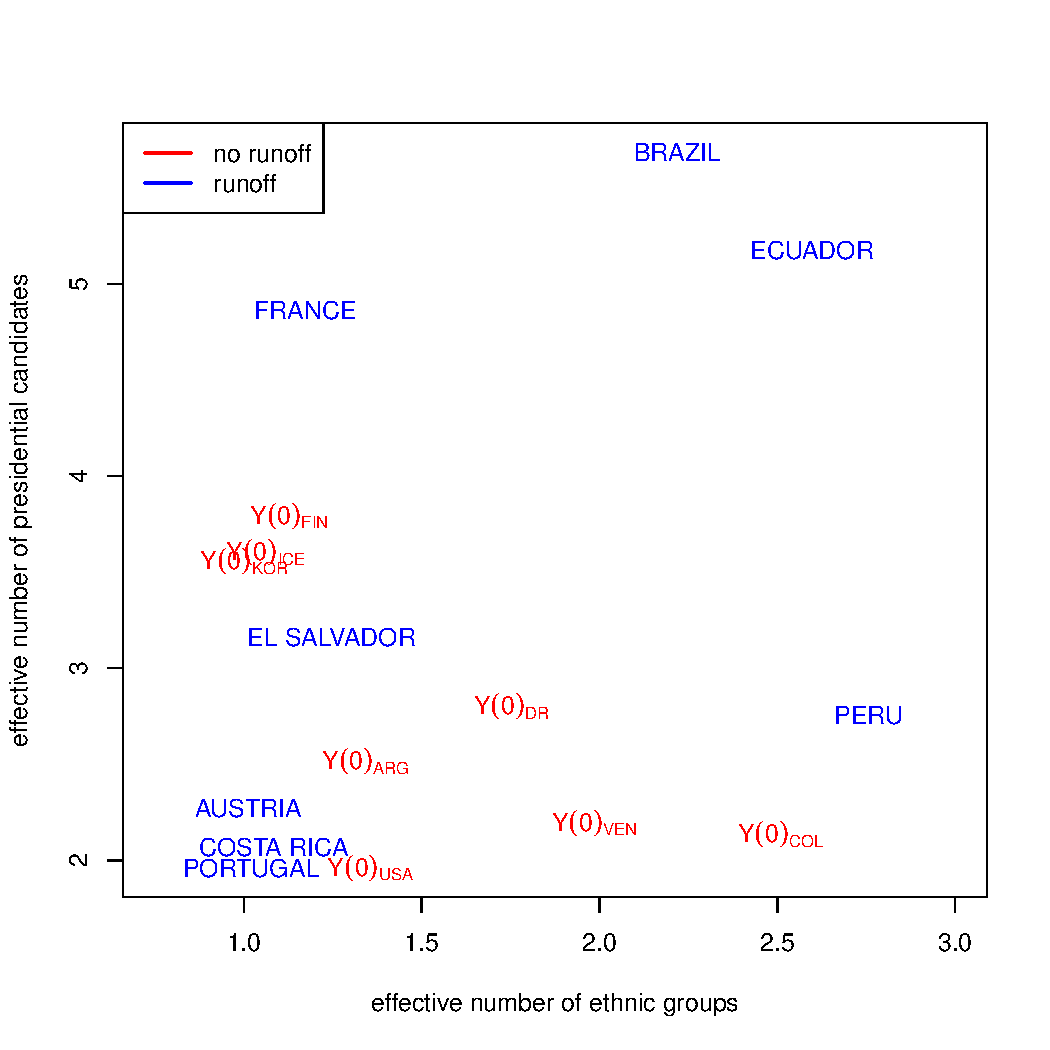
\includegraphics[height=3in]{figures/p1c.pdf}
  \end{center}
  \vspace{-0.275in}
\end{figure}

}

\frame{
\frametitle{Here is one way (with linear regression)}

\begin{figure}[ht]
  \begin{center}
    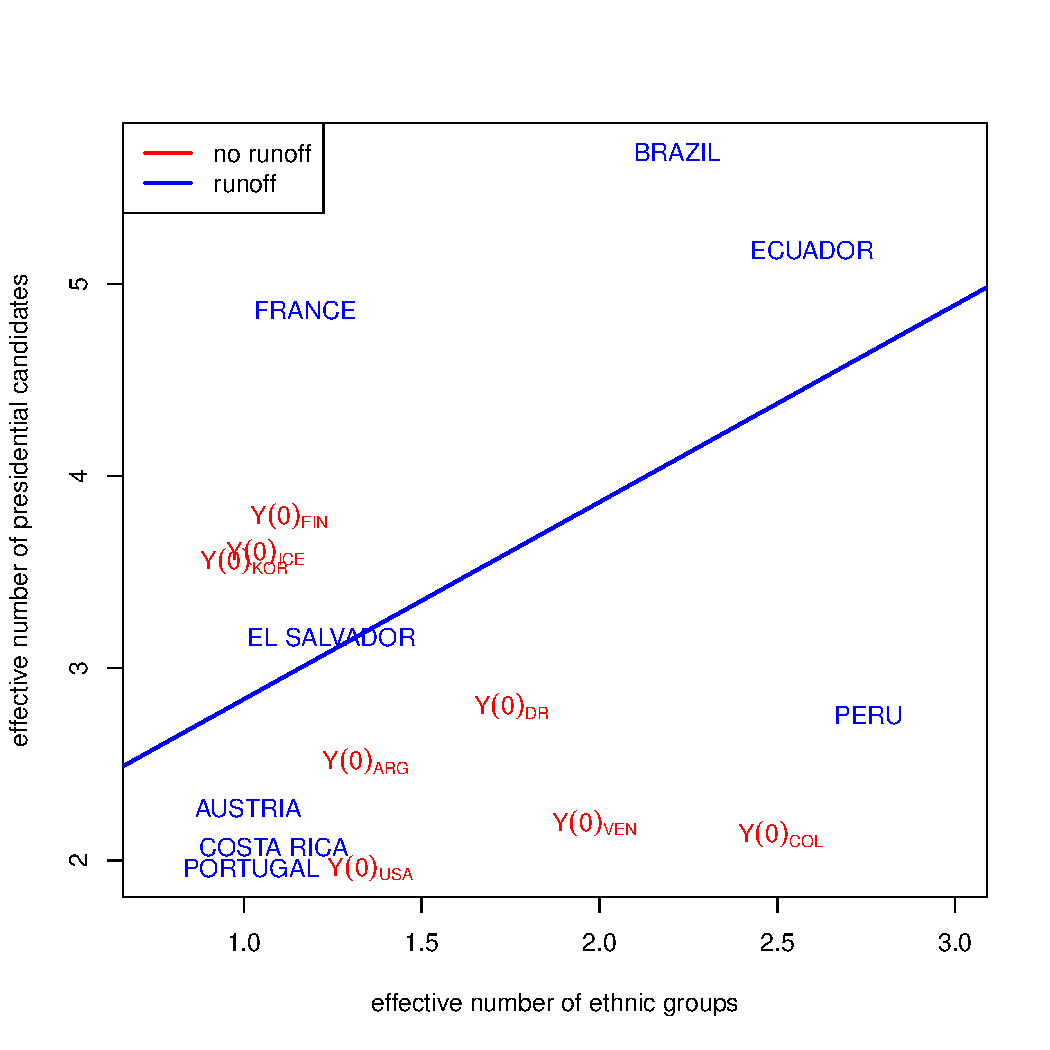
\includegraphics[height=3in]{figures/p1d.pdf}
  \end{center}
  \vspace{-0.275in}
\end{figure}

}

\frame{
\frametitle{Imputations on the line}

\begin{figure}[ht]
  \begin{center}
    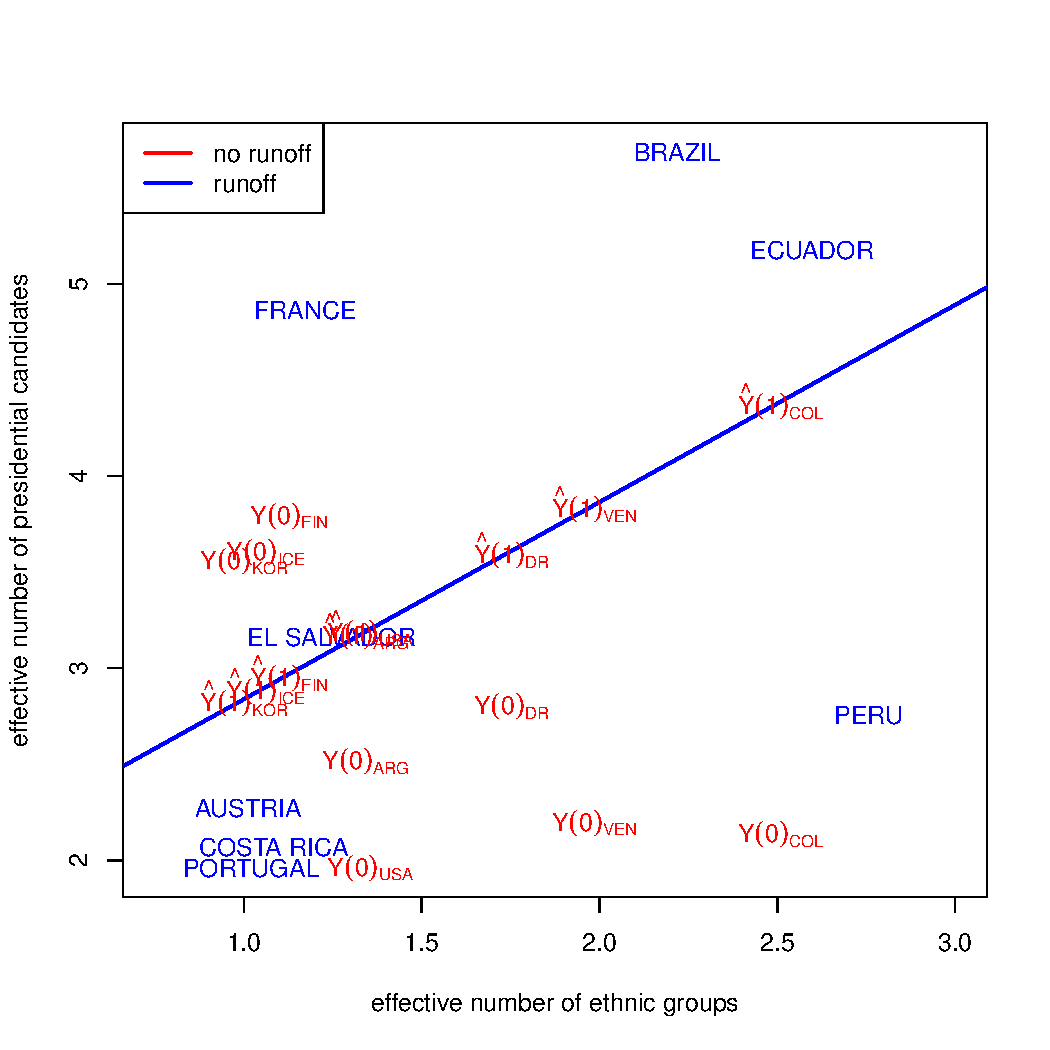
\includegraphics[height=3in]{figures/p1e.pdf}
  \end{center}
  \vspace{-0.275in}
\end{figure}

}



%\frame{
%\frametitle{Just like with missing "Drinking Water"}
%
%\begin{figure}[ht]
%  \begin{center}
%    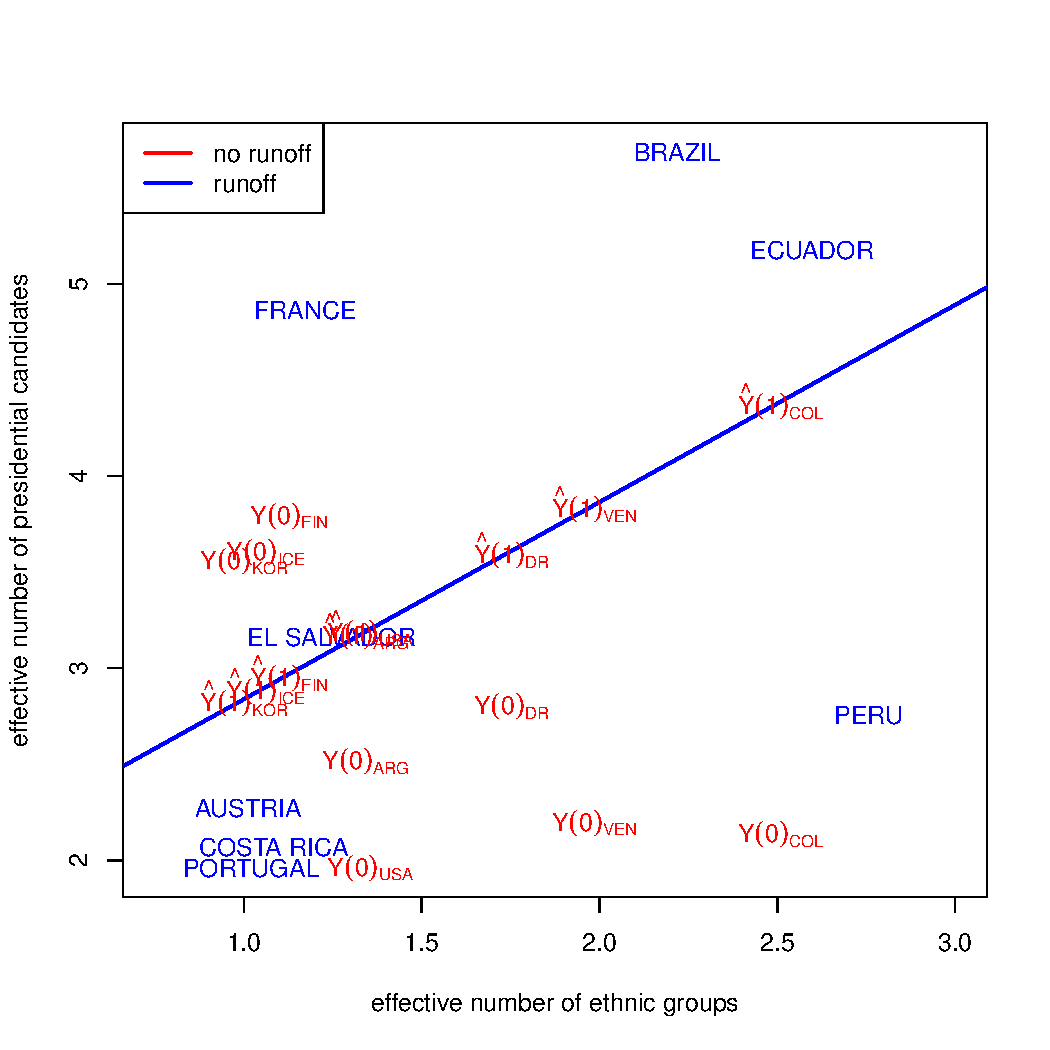
\includegraphics[height=3in]{figures/p1e.pdf}
%  \end{center}
%  \vspace{-0.275in}
%\end{figure}
%
%}


\frame{
\frametitle{Imputed Individual Treatment Effects}

\begin{figure}[ht]
  \begin{center}
    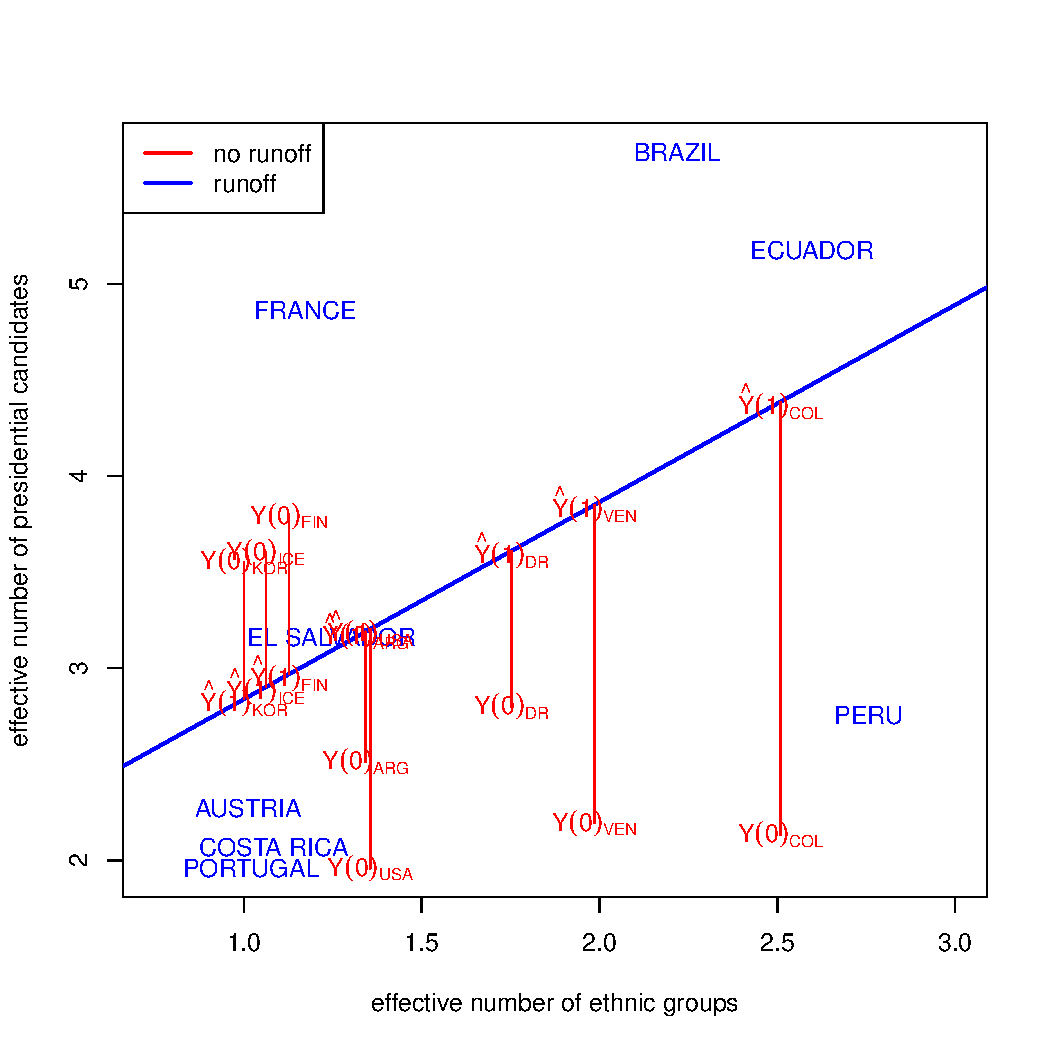
\includegraphics[height=3in]{figures/p1f.pdf}
  \end{center}
  \vspace{-0.275in}
\end{figure}

}



\frame{
\frametitle{An important identity (part 1)}

\begin{figure}[ht]
  \begin{center}
    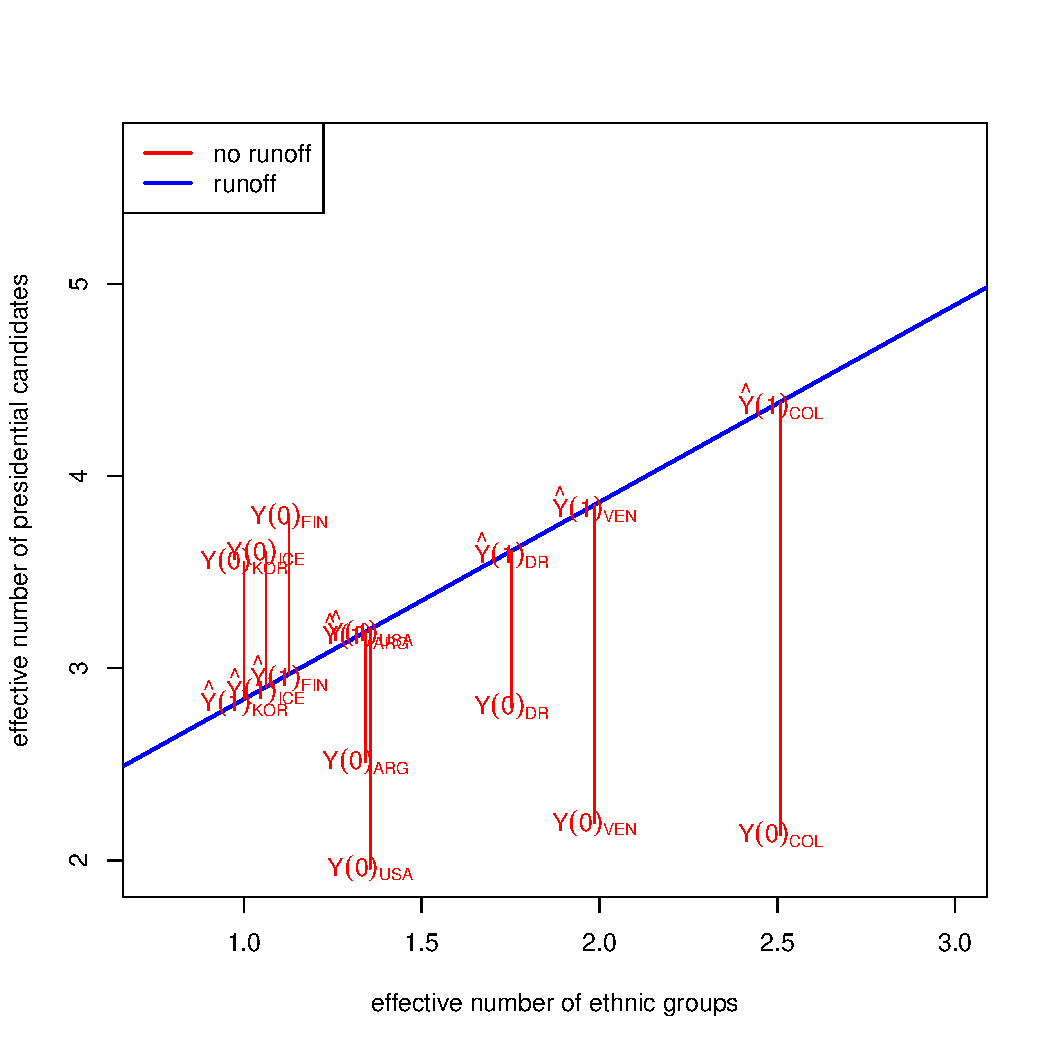
\includegraphics[height=3in]{figures/p1g.pdf}
  \end{center}
  \vspace{-0.275in}
\end{figure}

}

\frame{
\frametitle{An important identity (part 2)}

\begin{figure}[ht]
  \begin{center}
    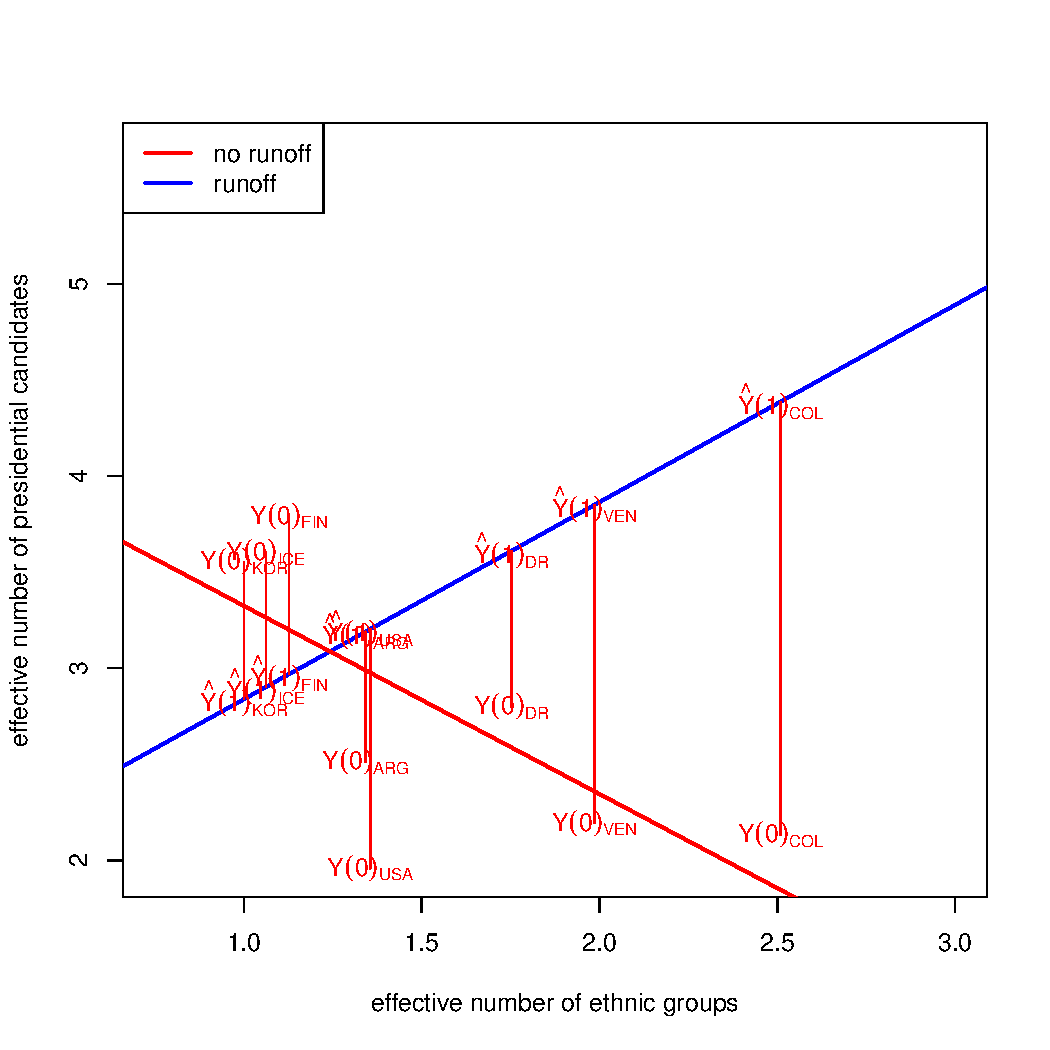
\includegraphics[height=3in]{figures/p1h.pdf}
  \end{center}
  \vspace{-0.275in}
\end{figure}

}

\frame{
\frametitle{An important identity (part 3)}

\begin{figure}[ht]
  \begin{center}
    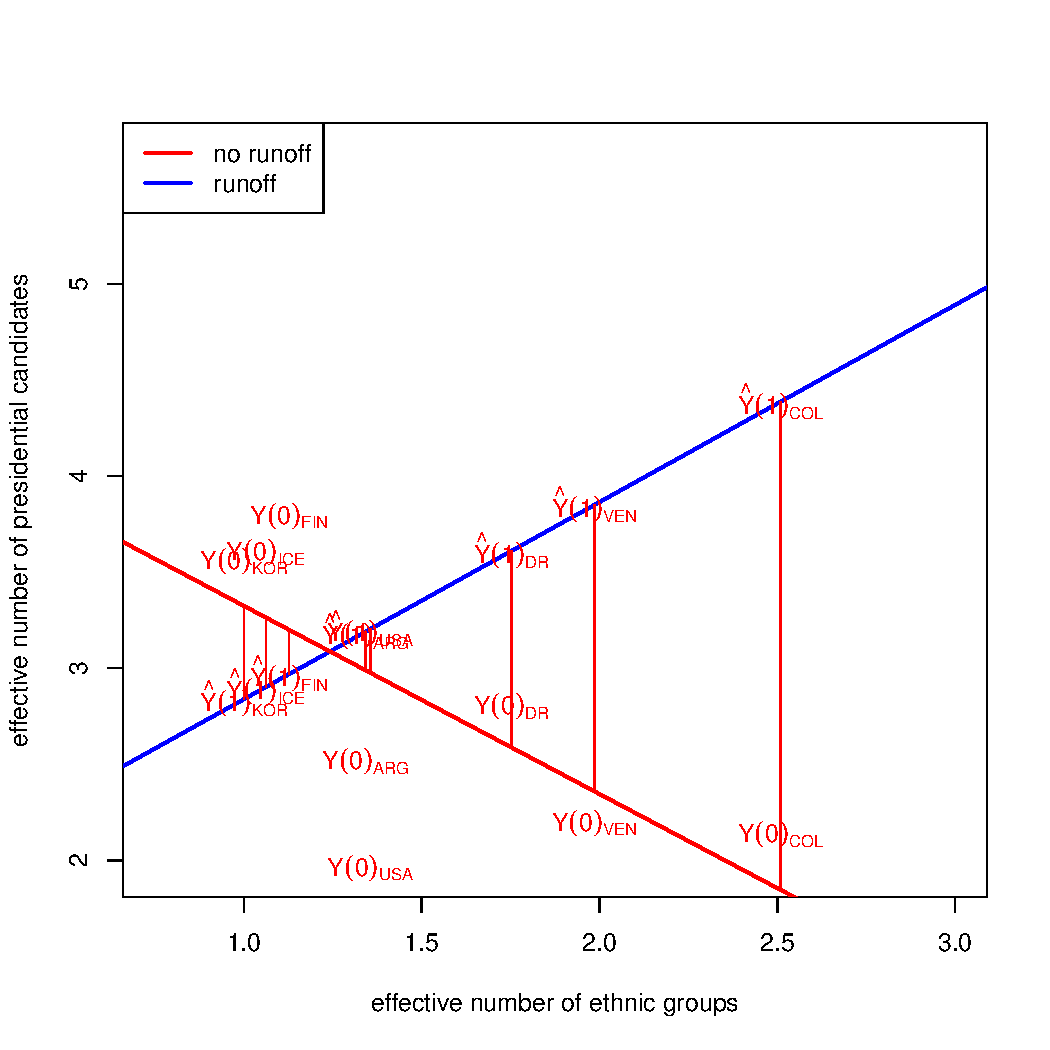
\includegraphics[height=3in]{figures/p1i.pdf}
  \end{center}
  \vspace{-0.275in}
\end{figure}

}

\frame{

... because the residuals sum to zero.
 
}

\frame{
\frametitle{$\widehat{ATE}$ among non runoff countries, equals ...}

\begin{figure}[ht]
  \begin{center}
    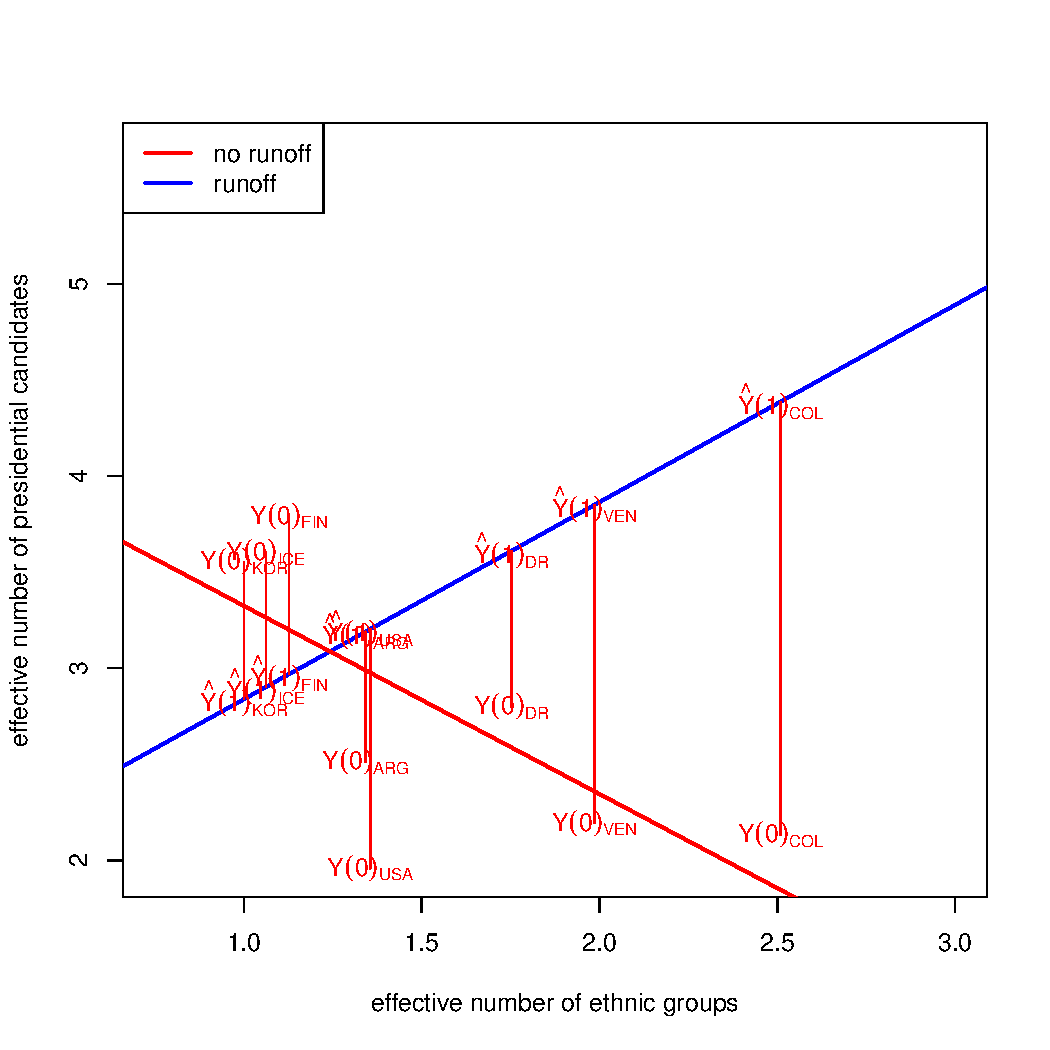
\includegraphics[height=3in]{figures/p1h.pdf}
  \end{center}
  \vspace{-0.275in}
\end{figure}

}

\frame{
\frametitle{$\widehat{APD}$ among non runoff countries}

\begin{figure}[ht]
  \begin{center}
    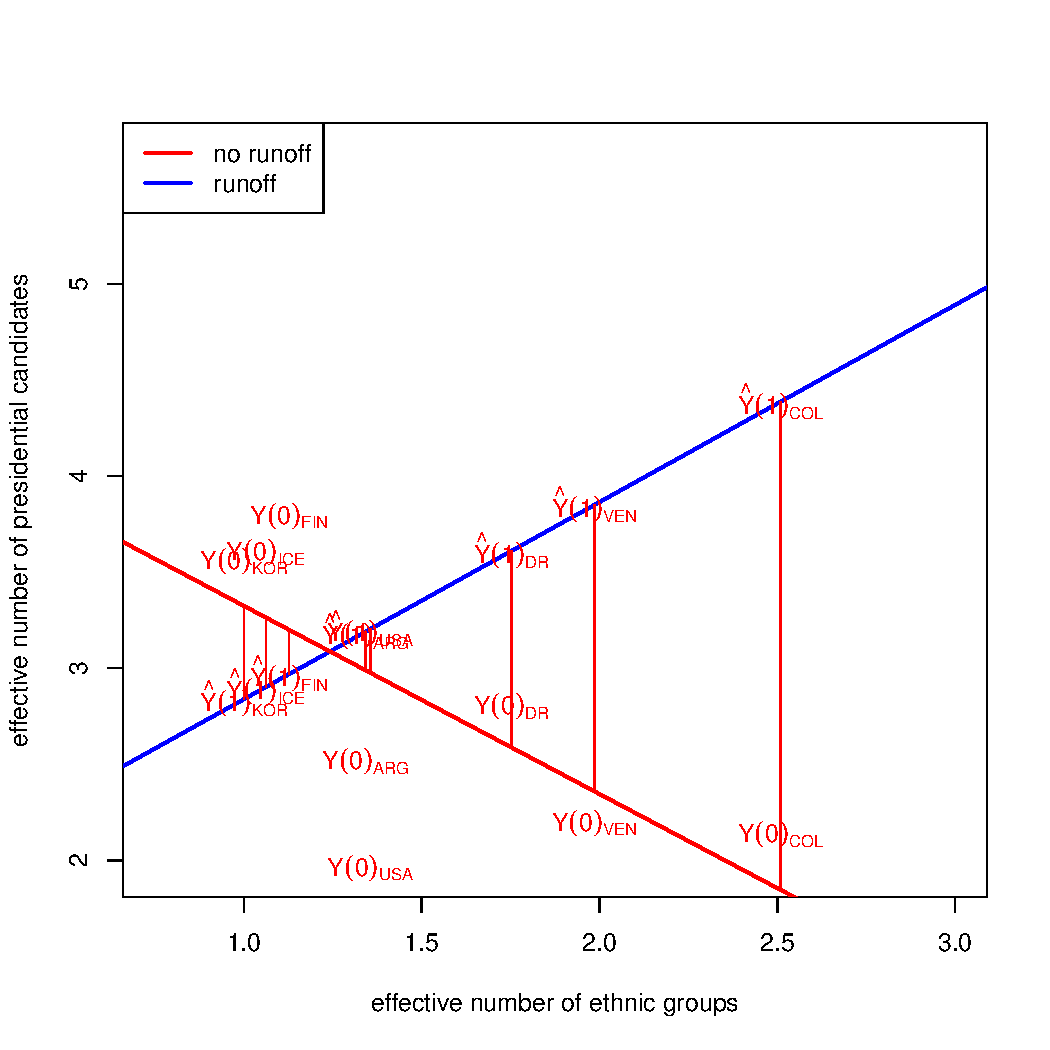
\includegraphics[height=3in]{figures/p1i.pdf}
  \end{center}
  \vspace{-0.275in}
\end{figure}

}

\frame{

This works the same way for the runoff countries, so the $\widehat{APD}$ equals the $\widehat{ATE}$

}


\frame{
\frametitle{$\widehat{APD}$ in Unpooled Linear Model ...}

\begin{figure}[ht]
  \begin{center}
%    \includegraphics<1>[height=3in]{figures/p3.pdf}
    \includegraphics<1>[height=3in]{figures/p4b.pdf}
  \end{center}
  \vspace{-0.275in}
\end{figure}

}

\frame{
\frametitle{... is the $\widehat{ATE}$ in Unpooled Linear Model}

\begin{figure}[ht]
  \begin{center}
 %   \includegraphics<1>[height=3in]{figures/p3.pdf}
    \includegraphics<1>[height=3in]{figures/p4b.pdf}
  \end{center}
  \vspace{-0.275in}
\end{figure}

}


\frame{

Omitted Variable Bias

}

\frame{

\begin{itemize}
\item we have been making the heroic assumption that whether a country has a runoff election is randomly assigned, conditional on how many ethnic groups they have.\pause
\item concerns about 1 are essentially concerns about omitted variable bias 
\end{itemize}

}

\begin{frame}
\frametitle{Recall this Omitted Variable Bias slide}

Suppose we want $B_1$ from $y_i=B_{0}+B_{1}x_{i}+B_{2}z_{i}+e_i$, but we run the regression of $y$ on $x$ alone. Suppose also that we have de-meaned $x_i$ and $z_i$ such that $\bar x = 0$ and $\bar z =0$. Then,
{\small
\begin{align*}
&\frac{\sum\limits_{i=1}^{n} x_i y_{i}}{\sum\limits_{i=1}^{n}x_i^2} = \visible<2->{\frac{\sum\limits_{i=1}^{n} x_i (B_{0}+B_{1}x_i+B_{2}z_i+e_i)}{\sum\limits_{i=1}^{n}x_i^2}}\\
&=\visible<3->{\frac{\sum\limits_{i=1}^{n}x_iB_{0}}{\sum\limits_{i=1}^{n}x_i^2}+\frac{\sum\limits_{i=1}^{n}x_iB_{1}x_i}{\sum\limits_{i=1}^{n}x_i^2}+\frac{\sum\limits_{i=1}^{n} x_i B_{2}z_i}{\sum\limits_{i=1}^{n}x_i^2} +\frac{\sum\limits_{i=1}^{n} x_i e_i}{\sum\limits_{i=1}^{n}x_i^2}  }\\
&= \visible<4->{ B_1+ B_2 \cdot  \frac{\sum\limits_{i=1}^{n}x_iz_i}{\sum\limits_{i=1}^{n}x_i^{2}} }
\end{align*}}

\end{frame}

\frame{
\frametitle{Potential Omitted Variables}


\begin{itemize}
\item colonial history?
\item ...
\end{itemize}
\pause


\bigskip

The omitted variable bias formulas we presented earlier give a ``back of the envelope'' method for considering the implications of omitted variables (see QTM electives for more precise approaches). 

}







\end{document}




%%%%%%%%%%%%%%%%%%%%%%%%%%%%%%

